\documentclass[12pt, twocolumn]{article}

%-------------------------------------------------------------------------------
% PACKAGES
%-------------------------------------------------------------------------------
\usepackage[super]{natbib}
\usepackage{mathtools}
\usepackage{nameref}
\usepackage{fancyref}
\usepackage[margin=0.7in]{geometry}

% section numbering
%\makeatletter
%\def\@seccntformat#1{%
%  \expandafter\ifx\csname c@#1\endcsname\c@section
%  \fi}
%\makeatother

% diagrams
\usepackage{tikz}
\usetikzlibrary{shapes,arrows,shadows}
\usepackage{amsmath,bm,times}
\newcommand{\mx}[1]{\mathbf{\bm{#1}}} % Matrix command
\newcommand{\vc}[1]{\mathbf{\bm{#1}}} % Vector command

%figures
\usepackage{caption}
\usepackage{subcaption}
\usepackage{epstopdf}
\usepackage{graphicx}
\graphicspath{{pictures/}}
\epstopdfsetup{outdir=pictures/}

%fancy stuff like color, paragraph formatting, code
\usepackage{hyperref}
\hypersetup{
     colorlinks   = true,
     citecolor    = gray
}
\usepackage{amsthm}
\usepackage{enumitem}
\setlist{nosep}
\usepackage{color, colortbl}
%one single command to rule them all references
\newcommand*{\fulleref}[1]{\hyperref[{#1}]{\autoref*{#1} \nameref*{#1}}} 
\usepackage{listings}
\usepackage{float}
\floatstyle{plain}
\restylefloat{figure}
\restylefloat{table}

%heading spacing
\usepackage{titlesec}
\setcounter{secnumdepth}{4}
\titlespacing\section{0pt}{12pt}{12pt}
\titlespacing\subsection{0pt}{8pt}{8pt}
\titlespacing\subsubsection{0pt}{8pt}{8pt}


\title{
\includegraphics[scale=0.1]{logos} \vspace*{3\baselineskip}\\
        \large \textbf{\textsc{Master's Thesis}} \\
        \normalsize \textsc{University of Rennes 1} \\
        \normalsize \textsc{Bioinformatics and genomics Master's Degree} \\
        \normalsize \textsc{(2014 - 2015)} \vspace*{2\baselineskip} \\
		\large \textbf{\textsc{Test and benchmarking of a new scaffolding methodology}} \vspace*{0.5\baselineskip}\\
		\footnotesize \textsc{Institute for Research in IT and Random Systems, Genscale \\
		263 Avenue General Leclerc, 35000 Rennes, France}
        }
\author{\normalsize
	\begin{minipage}{0.4\textwidth}
	\begin{flushleft} 
	\emph{Author:}\\
	\textsc{Alexandrina Bodrug}
	\end{flushleft}
	\end{minipage}
	~
	\begin{minipage}{0.4\textwidth}
	\begin{flushright}
	\emph{Supervisors:} \\
	\textit{Pr.} \textsc{Univ. Rennes 1 Rumen Andonov} \\
	\textit{Dr.} \textsc{Cnrs Dominique Lavenier}
	\end{flushright}
	\end{minipage}\\[2cm]}
\date{\small \textsc{22 June, 2015}}
\begin{document}
\maketitle
\thispagestyle{empty}
\clearpage
%-------------------------------------------------------------------------------
% THX
%-------------------------------------------------------------------------------
\onecolumn
Thanks \\
\thispagestyle{empty}
\clearpage
%-------------------------------------------------------------------------------
% ABBRV	 & GITHUB
%-------------------------------------------------------------------------------
\onecolumn
Abbreviations \& github link \\

\begin{itemize}
  \item \textit{Eucalyptus globulus} chloroplastic genome 
  \item \textit{Acorus calamus} chloroplastic genome
  \item \textit{Atropa belladonna} chloroplastic genome  
  \item \textit{Agrostis stolonifera} chloroplastic genome  
  \item \textit{Cucumis sativus} chloroplastic genome  
  \item \textit{Lecomlella madagascariensis} chloroplastic genome  
  \item \textit{Oenothera elata} chloroplastic genome  
  \item \textit{Pinus koraiensis} chloroplastic genome  
  \item \textit{Euglena gracilis} chloroplastic genome  
  \item \textit{Oryza sativa Japonica} chloroplastic genome  
\end{itemize}
\thispagestyle{empty}
\clearpage
%-------------------------------------------------------------------------------
% ToC
%-------------------------------------------------------------------------------
\hypersetup{linkcolor=gray}
\tableofcontents
\thispagestyle{empty}
\newpage
%-------------------------------------------------------------------------------
% BODEH!
%-------------------------------------------------------------------------------
%\twocolumn
\section{Introduction}
\setcounter{page}{1}
\subsection{Backgroud}
\textit{De novo} assembly is the process which pieces together overlapping small fragmented DNA sequences produced by Next Generation Sequencing methods into larger sequences. The aim is to obtain complete genomes (or chromosomes) containing gaps of known lengths because the less fragmented the genome is, the easier the downstream analysis are \cite{hunt_comprehensive_2014}. However an incomplete assembly is still sufficient for most of the analysis performed on DNA which explains why databases mainly contain partially assembled genomes. Nonetheless the uninterrupted genome sequence is a precious information and there has been an important effort made to improve the performance of assembly algorithms and the quality of NGS data. The the detailed process of assembly is described in ~\fulleref{sec:assterm}; the two main steps are building contigs from reads (sometimes referred to as assembly) and scaffolding, the ordering and relative orientation of contigs or unitigs. The 2011 and 2013 Assemblathon projects \cite{earl_assemblathon_2011} \cite{bradnam_assemblathon_2013} aimed at  benchmarking existing assembly tools with high coverage diploid genomes. The studies focused mainly on the contig building step, concluding that although many tools found quality assemblies, the tool and quality criteria should be adjusted to the type of genome and the goal of the assembly project. For example a good N50, an extensively used metric which is the contig length such that using equal or longer contigs produces half the bases of the genome, is not essential in a gene detecting assembly project. \\
The first stand-alone scaffolder named Bambus \cite{pop_hierarchical_2004}, originally part of the MetAMOS \cite{treangen_metamos:_2013} assembly and analysis pipeline, was published in 2004. Previously the scaffolding step was missing or presented as an option within conting builders, for instance the Velvet\cite{zerbino_velvet:_2008} assembler \textit{'scaffolding yes or no'} option. In the 2014 comprehensive evaluation of scaffolding tools \cite{hunt_comprehensive_2014-1}, Hunt \textit{et al} found that no tool identified more than 90\% of joins between real-data Velvet assembled contigs, meaning genomes were still fragmented into many scaffolds as joins were missing for a complete and accurate ordering and orientation. The study also used simulated data highlighting the fact that perfect data doesn't always yield perfect results. Despite its simply formulated goal - order and orient contigs - scaffolding is a challenging computational problem. It was first described and modeled in 2002 by Hudson \textit{et al.}\cite{huson_greedy_2002} which proposed a greedy path-merging strategy, described in \fulleref{sec:hiscaf} along with other proposed algorithms.
 
\subsection{Assembly terminology}\label{sec:assterm}
In this report \textit{assembly} will refer to the whole multi-step process which starts from once filtered out-of-the-sequencer data and results, in the best case scenarios, in  highly uninterrupted sequence of a genome or chromosome. As previously mentioned, the two main steps are contig/unitig building and contig/unitg scaffolding. The difference between contig and unitig is fundamental to understanding the Genscale scaffolding challenges. Another key point is the construction of joins between contigs/unitigs - also referred to as links, edges, bonds \ldots 
\subsubsection{Reads, pairing and overlaps} \label{sec:rpao}

A read is a short ($<500pb$) copy of a DNA fragment of known length and nucleic acid order. It is produced differently depending of the sequencing technology. Paired reads are copies of the two extremities of a DNA molecule. The DNA sequence between two reads of a pair is called an insert. The size of the insert is variable. Reads with small insert sizes ($<500bp$) are called paired-end reads. Mate-paired reads are reads whose insert size is very big (up to tens of kilobases). The pairing information and the size of the insert are provided by the sequencer. A collection of reads with their associated insert size is called a a genomic library.
\begin{figure}[h!]
%\resizebox{5in}{!}{
\hspace*{3cm}
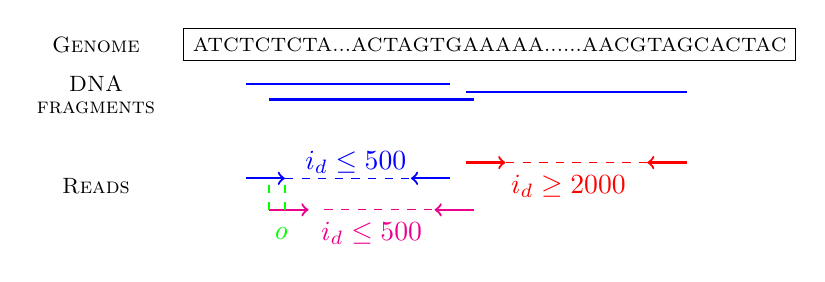
\begin{tikzpicture}
\node[draw=none] at (-4,0) {\footnotesize \textsc{Genome}};
\node[draw] at (1,0) {\scriptsize ATCTCTCTA...ACTAGTGAAAAA......AACGTAGCACTAC};
\node[draw=none] at (-4,-0.5) {\footnotesize \textsc{DNA}};
\node[draw=none] at (-4,-0.8) {\footnotesize \textsc{fragments}};
\draw[thick, blue] (-2.1, -0.5) -- (0.5, -0.5);
\draw[thick, blue] (0.7, -0.6) -- (3.5, -0.6);
\draw[thick, blue] (-1.8, -0.7) -- (0.8, -0.7);
\node[draw=none] at (-4,-1.8) {\footnotesize \textsc{Reads}};

\draw[red, thick, <-] (3,-1.5) -- (3.5,-1.5);
\draw[red, dashed] (3,-1.5) -- (1.2,-1.5);
\node[draw=none, color=red] at (2,-1.8) {\textit{$i_d \geq 2000$}};
\draw[red, thick, ->] (0.7,-1.5) -- (1.2,-1.5);

\draw[blue, thick, <-] (0,-1.7) -- (0.5,-1.7);
\draw[blue, dashed] (-1.6,-1.7) -- (0,-1.7);
\node[draw=none, color=blue] at (-0.7,-1.5) {\textit{$i_d\leq 500$}};
\draw[blue, thick, ->] (-2.1,-1.7) -- (-1.6,-1.7);

\draw[magenta, thick, <-] (0.3,-2.1) -- (0.8,-2.1);
\draw[magenta, dashed] (-1.1,-2.1) -- (0.3,-2.1);
\node[draw=none, color=magenta] at (-0.5,-2.4) {\textit{$i_d\leq 500$}};
\draw[magenta, thick, ->] (-1.8,-2.1) -- (-1.3,-2.1);

\node[draw=none, color=green] at (-1.65, -2.4) {\textit{o}};
\draw[green, dashed, thick] (-1.8, -2.1) -- (-1.8, -1.7); 
\draw[green, dashed, thick] (-1.6, -2.1) -- (-1.6, -1.7);
\end{tikzpicture}
%}
\caption{Alignment of paired reads on fragmented DNA}
\label{fig:reads}
{\scriptsize  Each end of a DNA molecule is cloned to produce paired reads. Here is represented a mate-paired pair (red) with a big insert size \textit{($i_d$)} and two paired-end pairs (blue and magenta) which slightly overlap \textit{(o)}. }
\end{figure}\\
Figure \ref{fig:reads} represents three pairs of reads. Within the pairs, reads are facing each other: this configuration is called \textit{Forward-Reverse} read orientation. To be sequenced the genome represented in figure \ref{fig:reads} is first amplified by Polymerase Chain Reaction and then fragmented into numerous DNA molecules by sonication or nebulization. Each end of the molecule is then cloned. Overlapping of reads occurs when two reads sequence a portion of the same genomic region, but not only. The overlapping concept implies a common origin but unfortunately overlapping can occur if two reads sequence two different repeated genomic regions. Figure \ref{fig:overlapping} shows how repeated regions create false positive overlaps. Such reads can be detected and filtered out by ignoring high-frequency overlaps (higher than the coverage at which the genome was sequenced). However this can result in false negatives and makes the task of assembling repeated regions very hard.
\begin{figure}[h!]
\hspace*{4cm}
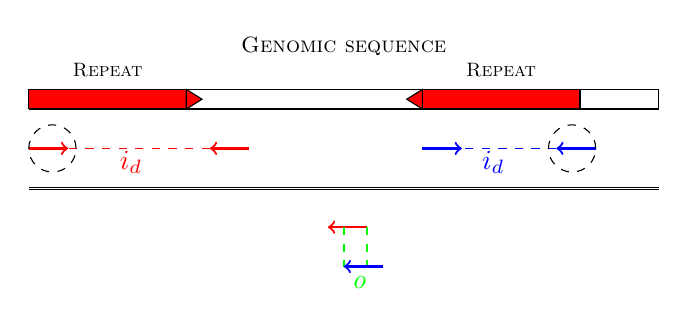
\begin{tikzpicture}
\node[draw=none] at (4,0.8) {\footnotesize \textsc{Genomic sequence}};
\node[draw=none] at (1,0.5) {\scriptsize \textsc{Repeat}};
\node[draw=none] at (6,0.5) {\scriptsize \textsc{Repeat}};
\draw[fill=red] (0,0) -- (2,0) -- (2,0.25) -- (0,0.25) -- (0,0);
\draw[fill=red] (2,0) -- (2,0.25) -- (2.2,0.125) -- (2,0);
\draw (2,0) -- (5,0) -- (5,0.25) -- (2,0.25) -- (2,0);
\draw[fill=red] (5,0) -- (5,0.25) -- (4.8,0.125) -- (5,0);
\draw[fill=red] (5,0) -- (7,0) -- (7,0.25) -- (5,0.25) -- (5,0);
\draw (7,0) -- (8,0) -- (8,0.25) -- (7,0.25) -- (7,0);

\draw[red, thick, <-] (2.3,-0.5) -- (2.8,-0.5);
\draw[red, dashed] (2.3,-0.5) -- (0.2,-0.5);
\node[draw=none, color=red] at (1.3,-0.68) {\textit{$i_d$}};
\draw[red, thick, ->] (0,-0.5) -- (0.5,-0.5);

\draw[blue, thick, <-] (6.7,-0.5) -- (7.2,-0.5);
\draw[blue, dashed] (6.7,-0.5) -- (5.2,-0.5);
\node[draw=none, color=blue] at (5.9,-0.68) {\textit{$i_d$}};
\draw[blue, thick, ->] (5,-0.5) -- (5.5,-0.5);

\draw[dashed] (0.3,-0.5) circle (0.3) ; 
\draw[dashed] (6.9,-0.5) circle (0.3) ; 

\draw (0,-1)-- (8,-1) ;
\draw (0,-1.02)-- (8,-1.02) ;

\draw[red, thick, ->] (4.3,-1.5) -- (3.8,-1.5);
\draw[green, thick, dashed] (4, -1.5) -- (4, -2);
\draw[green, thick, dashed] (4.3, -1.5) -- (4.3, -2);
\draw[blue, thick, ->] (4.5,-2) -- (4,-2);
\node[draw=none, color=green] at (4.2, -2.2) {\textit{o}};

\end{tikzpicture}
\caption{Overlapping induced by repeated sequences}
\label{fig:overlapping}
{\scriptsize  The two circled reads will have a significantly long and accurate overlap to imply a common genomic origin when in fact they come from distant regions.}
\end{figure}

\subsubsection{Unitigs and Contigs}
Unitigs are an uniquely assemblable subset of overlapping fragments. At the end of an unitig data shows multiple dubious overlaps as seen in \fulleref{sec:rpao} creating joins with multiple other unitigs. Contigs are larger than unitigs, extended through repeat boundaries but are still ungapped sequences. Contigs are interesting to construct because there is a higher chance to detect genes. 
Taking the example shown in figure \ref{fig:overlapping}, a contig will merge the first three DNA fragments and will then be extended though the ambiguous overlaps, merging the red DNA fragments' sequence. Unitigs however will stop at the end of the third DNA fragment and assemble the red fragments separately. In a sense, unitigs are either an unambiguous contig or a compression of several copies of a repeat. The advantage of working with unitigs is that there are less chances of erroneous merging of two far away genomic regions. This feature is used in the Genscale scaffolding strategy, further discussed in \fulleref{sec:genscafmeth}.

\begin{figure}[h!]
\resizebox{5in}{!}{
\hspace*{2cm}
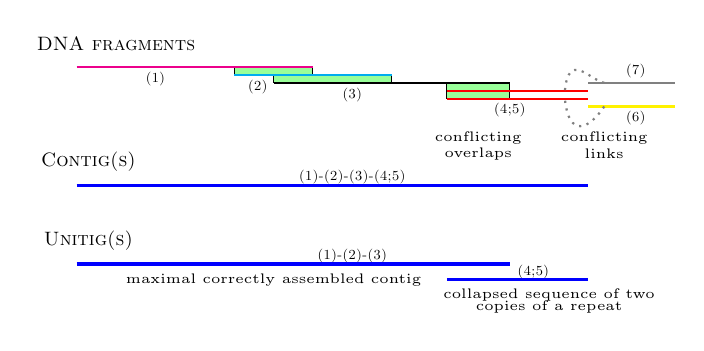
\begin{tikzpicture}
\node[draw=none] at (1,0.3) {\scriptsize \textsc{DNA fragments}};
\node[draw=none] at (1.5,-0.15) {\tiny \textsc{(1)}};
\node[draw=none] at (2.8,-0.25) {\tiny \textsc{(2)}};
\node[draw=none] at (4,-0.35) {\tiny \textsc{(3)}};
\node[draw=none] at (6,-0.55) {\tiny \textsc{(4;5)}};
\node[draw=none] at (7.6,-0.65) {\tiny \textsc{(6)}};
\node[draw=none] at (7.6,-0.05) {\tiny \textsc{(7)}};
\node[draw=none] at (4,-1.4) {\tiny \textsc{(1)-(2)-(3)-(4;5)}};
\node[draw=none] at (4,-2.4) {\tiny \textsc{(1)-(2)-(3)}};
\node[draw=none] at (6.3,-2.6) {\tiny \textsc{(4;5)}};

\draw[fill=green!40] (2.5,0) -- (3.5,0) -- (3.5,-0.1) -- (2.5,-0.1) -- (2.5,0);
\draw[fill=green!40] (3,-0.1) -- (4.5,-0.1) -- (4.5,-0.2) -- (3,-0.2) -- (3,-0.1);
\draw[fill=green!40] (5.2,-0.2) -- (6.0,-0.2) -- (6.0,-0.3) -- (5.2,-0.3) -- (5.2,-0.2);
\draw[fill=green!40] (5.2,-0.3) -- (6.0,-0.3) -- (6.0,-0.4) -- (5.2,-0.4) -- (5.2,-0.3);

\draw[thick, magenta] (0.5,0) -- (3.5,0);
\draw[thick, cyan] (2.5,-0.1) -- (4.5,-0.1);
\draw[thick, black] (3.0,-0.2) -- (6.0,-0.2);
\draw[thick, red] (5.2,-0.3) -- (7,-0.3);
\draw[thick, red] (5.2,-0.4) -- (7,-0.4);
\draw[thick, yellow!] (7.0,-0.5) -- (8.1,-0.5);
\draw[thick, gray] (7.0,-0.2) -- (8.1,-0.2);

\draw[color=gray, dotted, thick] (7.2,-0.2) .. controls  (7,-0.15) and (6.75,0.2) .. (6.7,-0.3);
\draw[color=gray, dotted, thick] (7.2,-0.5) .. controls  (7,-0.8) and (6.75,-0.9) .. (6.7,-0.4);

\node[draw=none] at (5.6,-0.9) {\tiny conflicting};
\node[draw=none] at (5.6,-1.1) {\tiny overlaps};
\node[draw=none] at (7.2,-0.9) {\tiny conflicting};
\node[draw=none] at (7.2,-1.1) {\tiny links};
\node[draw=none] at (0.65,-1.2) {\scriptsize \textsc{Contig(s)}};
\draw[very thick, blue] (0.5, -1.5) -- (7, -1.5);
\node[draw=none] at (0.65,-2.2) {\scriptsize \textsc{Unitig(s)}};
\draw[very thick, blue] (0.5, -2.5) -- (6.0, -2.5);
\node[draw=none] at (3,-2.7) {\tiny maximal correctly assembled contig};
\draw[very thick, blue] (5.2, -2.7) -- (7, -2.7);
\node[draw=none] at (6.5,-2.9) {\tiny collapsed sequence of two };
\node[draw=none] at (6.5,-3.05) {\tiny copies of a repeat};
\end{tikzpicture}
}
\caption{The difference between unitigs and contigs}
\label{fig:unitgscontigs}
{\scriptsize Unitigs end at multiple overlaps indicating a possible repeat. Contigs can be extended through conflicting overlaps. Here, the red DNA fragments are two copies of a repeat. When no more overlaps exist, contigs can be linked (gray dotted line) thanks to information provided by read pairs. This is the scaffolding task. Here alternative paths are possible due to the repeated region.}
\end{figure}
\newpage
\subsubsection{Obtaining scaffolds}
A scaffold is a linear ordering of contigs (or unitigs). The ordering and relative orientation of contigs is possible thanks to paired reads information. The first step of scaffolding is mapping reads on the previously constructed contigs: the two most used mappers are bwa \cite{li_fast_2009} and bowtie\cite{langmead_fast_2012,langmead_ultrafast_2009}. A pair of reads mapping on two different contigs provide a join, which holds the information of distance between the two contigs, and relative orientation (see figure \ref{fig:mappreads}).  A same contig can have joins with multiple  other contigs (see \textsc{conflicting joins} figure \ref{fig:unitgscontigs} and \textsc{created joins} figure \ref{fig:mappreads}). These multiple joins which result in multiple paths when ordering and orienting contigs are solved differently by scaffolders. Most of the time, a choice is made - heuristically - to use one join over another. Another strategy is illustrated in figure \ref{fig:mappreads}, where the contig with the two high-confidence joins is duplicated. This is the strategy of the Genscale scaffolders, further described in \fulleref{sec:genscafmeth}. \\
The concept of insert size is essential to understand the challenges of scaffolding when dealing with repeated regions in genomes. Take \textsc{contig (1)} and \textsc{contig (2)} in figure \ref{fig:mappreads}: the two contigs are separated by a gap of undefined size. Say this gap is caused by a repeated region where reads mapped multiple times and were thus discarded, or the region wasn't sequenced by the sequencer and is all together absent. If the region is bigger than the insert size, no read pair will span over it. The join between contig (1) and contig (2) will not exist. This explains why mate-pair information is extremely useful. When multiple mate-pair libraries with different big insert size are available, genomically distanced regions can directly be ordered and orientated. The scaffolds will potentially be longer, as missing or ambiguous data doesn't impede its construction.

\begin{figure}[h!]
\resizebox{5in}{!}{
\hspace*{4cm}
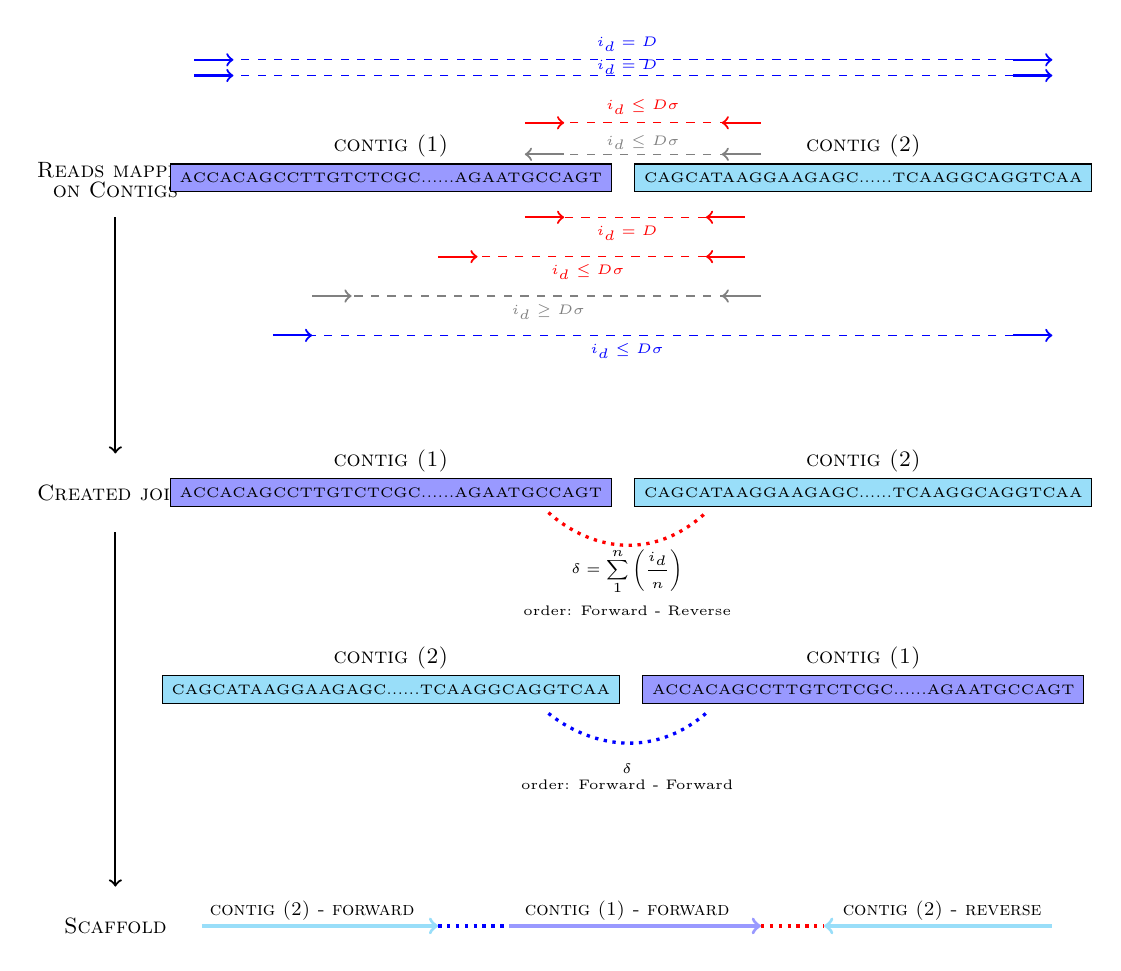
\begin{tikzpicture}
\node[draw=none] at (-2.5,-1.4) {\footnotesize \textsc{Reads mapped}};
\node[draw=none] at (-2.5,-1.65) {\footnotesize \textsc{on Contigs}};
\node[draw, fill=blue!40] at (1,-1.5) {\tiny ACCACAGCCTTGTCTCGC......AGAATGCCAGT};
\node[draw, fill=cyan!40] at (7,-1.5) {\tiny CAGCATAAGGAAGAGC......TCAAGGCAGGTCAA};
%red reads
\draw[red, thick, <-] (5,-2) -- (5.5,-2);
\draw[red, dashed] (5,-2) -- (3.2,-2);
\node[draw=none, color=red] at (4.0,-2.2) {\tiny {$i_d=D$}};
\draw[red, thick, ->] (2.7,-2) -- (3.2,-2);
%red reads
\draw[red, thick, <-] (5,-2.5) -- (5.5,-2.5);
\draw[red, dashed] (5,-2.5) -- (2.1,-2.5);
\node[draw=none, color=red] at (3.5,-2.7) {\tiny {$i_d\leq D\sigma$}};
\draw[red, thick, ->] (1.6,-2.5) -- (2.1,-2.5);
%red reads
\draw[red, thick, <-] (5.2,-0.8) -- (5.7,-0.8);
\draw[red, dashed] (5.7,-0.8) -- (3.2,-0.8);
\node[draw=none, color=red] at (4.2,-0.6) {\tiny {$i_d\leq D\sigma$}};
\draw[red, thick, ->] (2.7,-0.8) -- (3.2,-0.8);
%pink reads
\draw[gray, thick, <-] (5.2,-1.2) -- (5.7,-1.2);
\draw[gray, dashed] (5.7,-1.2) -- (3.2,-1.2);
\node[draw=none, color=gray] at (4.2,-1.05) {\tiny {$i_d\leq D\sigma$}};
\draw[gray, thick, ->] (3.2,-1.2) -- (2.7,-1.2);
%pink reads
\draw[gray, thick, <-] (5.2,-3) -- (5.7,-3);
\draw[gray, dashed] (5.7,-3) -- (0.5,-3);
\node[draw=none, color=gray] at (3,-3.2) {\tiny {$i_d\geq D\sigma$}};
\draw[gray, thick, ->] (0,-3) -- (0.5,-3);
%blue reads
\draw[blue, thick, <-] (9.4,0) -- (8.9,0);
\draw[blue, dashed] (8.9,0) -- (-1,0);
\node[draw=none, color=blue] at (4,0.2) {\tiny {$i_d=D$}};
\draw[blue, thick, ->] (-1.5,0) -- (-1,0);
%blue reads
\draw[blue, thick, <-] (9.4,-0.2) -- (8.9,-0.2);
\draw[blue, dashed] (8.9,-0.2) -- (-1,-0.2);
\node[draw=none, color=blue] at (4,-0.1) {\tiny {$i_d=D$ }};
\draw[blue, thick, ->] (-1.5,-0.2) -- (-1,-0.2);
%blue reads
\draw[blue, thick, <-] (9.4,-3.5) -- (8.9,-3.5);
\draw[blue, dashed] (8.9,-3.5) -- (0,-3.5);
\node[draw=none, color=blue] at (4,-3.7) {\tiny {$i_d\leq D\sigma$}};
\draw[blue, thick, ->] (-0.5,-3.5) -- (0,-3.5);
\node[draw=none] at (1,-1.1) {\footnotesize \textsc{contig (1)}};
\node[draw=none] at (7,-1.1) {\footnotesize \textsc{contig (2)}};

\begin{scope}[shift={(0,-1)}]
\node[draw=none] at (-2.5,-4.5) {\footnotesize \textsc{Created joins}};
\node[draw, fill=blue!40] at (1,-4.5) {\tiny ACCACAGCCTTGTCTCGC......AGAATGCCAGT};
\node[draw, fill=cyan!40] at (7,-4.5) {\tiny CAGCATAAGGAAGAGC......TCAAGGCAGGTCAA};
\draw[thick, ->] (-2.5, -1) -- (-2.5, -4);
\draw[color=red, dotted, very thick] (3,-4.75) .. controls  (3.5,-5.2) and (4.3,-5.4) .. (5,-4.75);
\node[draw=none] at (4,-5.5) {\tiny $\delta = \displaystyle\sum_{1}^{n}{\left(\frac{i_d}{n}\right)}$};

\node[draw=none] at (4,-6) {\tiny order: Forward - Reverse};

\node[draw, fill=cyan!40] at (1,-7) {\tiny CAGCATAAGGAAGAGC......TCAAGGCAGGTCAA};
\node[draw, fill=blue!40] at (7,-7) {\tiny ACCACAGCCTTGTCTCGC......AGAATGCCAGT};
\draw[color=blue, dotted, very thick] (3,-7.3) .. controls  (3.5,-7.7) and (4.3,-7.9) .. (5,-7.3);
\node[draw=none] at (4,-8) {\tiny $\delta$};
\node[draw=none] at (4,-8.2) {\tiny order: Forward - Forward};

\node[draw=none] at (1,-4.1) {\footnotesize \textsc{contig (1)}};
\node[draw=none] at (1,-6.6) {\footnotesize \textsc{contig (2)}};
\node[draw=none] at (7,-4.1) {\footnotesize \textsc{contig (2)}};
\node[draw=none] at (7,-6.6) {\footnotesize \textsc{contig (1)}};
%SCAFFOLD PART
\node[draw=none] at (0,-9.8) {\scriptsize \textsc{contig (2) - forward}};
\node[draw=none] at (4,-9.8) {\scriptsize \textsc{contig (1) - forward}};
\node[draw=none] at (8,-9.8) {\scriptsize \textsc{contig (2) - reverse}};
\node[draw=none] at (-2.5,-10) {\footnotesize \textsc{Scaffold}};
\draw[thick, ->] (-2.5, -5) -- (-2.5, -9.5);
\draw[very thick, ->, color=cyan!40] (-1.4,-10) -- (1.6, -10);
\draw[very thick, dotted, color=blue] (1.6,-10) -- (2.5, -10);
\draw[very thick, ->, color=blue!40] (2.5,-10) -- (5.7, -10);
\draw[very thick, dotted, color=red] (5.7,-10) -- (6.5, -10);
\draw[very thick, <-, color=cyan!40] (6.5,-10) -- (9.4, -10);
\end{scope}

\end{tikzpicture}
}
\caption{Creating joins between contigs thanks to read pair information}
\label{fig:mappreads}
{\scriptsize {\color{magenta}$i_d:$} insert size , {\color{magenta}$D:$} expected insert size , {\color{magenta}$\sigma:$} distance standard deviation , {\color{magenta}$n:$} number of retained correctly mapped paired reads for the join, {\color{magenta}$\delta$} estimated distance.\\
Paired reads are mapped on previously assembled contigs. Pairs with reads mapping on different contigs provide linking information. The library represented is Forward - Reverse (reads are facing each other, see {\color{red}red pairs}). Additional read pairs with a satisfying $i_d$ but with a different orientation can coexist with the Foward - Reverse pairs (here, {\color{blue}blue pairs}, Forward - Forward). Pairs which map with a big insert size ($\geq D3\sigma$) are usually discarded (here, {\color{gray}gray pairs}). Red and blue pairs are retained to create two conflicting joins between \textsc{contig (1)} and \textsc{contig (2)}. The conflict can be solve with a scaffolder which duplicated \textsc{contig (2)} allowing both joins to coexist, or ignoring one of the joins (not represented).\\
%Red: contig (1) Forward - contig (2) Reverse \\
%Blue: contig (2) Forward - contig (1) Forward
}
\end{figure}

\newpage
\subsection{A history of scaffolding strategies}\label{sec:hiscaf}
The scaffolding problem was first introduced in 2002 by Hudson \textit{et al.} \cite{huson_greedy_2002} following the challenges which arose during the human genome clone-by-clone sequencing by \textit{Lander et al.} \cite{lander_initial_2001} and the human whole genome shotgun  assembly project by Venter \textit{et al.} \cite{venter_sequence_2001-1}, both published in 2001. The Hudson \textit{et al.} paper defines the problem as follows: "The \textit{Contig Scaffolding Problem}  is to order and orientate the given contigs in a manner that is consistent with as many mate-pairs as possible". The problem is modeled as a graph where vertices represent contigs and links represent bundles of pairs of reads joining two contigs (see figure \ref{fig:mappreads}, red and blue pairs are bundled into two joins which will be represented by a link in the graph). This model is reused in most of the stand alone scaffolding tools. 

\subsubsection{Examples of scaffolding tools using heuristics}
Hudson et al, SSPACE, Bambus
\subsubsection{Examples of scaffolding tools solving the problem exactly}
Opera, SGA, SOPRA
\subsubsection{Characteristics of the Genscale scaffolding tools}
Several models have been developed and tested. Among them: distance based and weighted path models. A new multi-step called flow model is in development. Each processes the same type of data which is different than what is given to the previously described scaffolders.

\iffalse
 Erroneous data (fake links due to poorly assembled contigs, low quality libraries), missing data (low quality libraries, unfit insert size, low genome coverage) and inherent genome characteristics (repeated regions,  heterozygosity) stand in the way of a perfect and easy scaffolding process.
\fi
\subsection{Goal of the internship project}
The goal of this report is present the performance of the Genscale scaffolding tools (GST) with reliable simulated data and some instances of real data. The first step is to compare the solutions obtained by GST with available solutions. The second step is to benchmark the GST against published tools. In order to achieve this task, a benchmarking workflow was set up and is described in \fulleref{sec:benchmarking} of \fulleref{sec:MatMet}. The data format and data type are described in \fulleref{sec:genscafmeth} of \fulleref{sec:MatMet}.
\ldots

\iffalse
Describe all parts, annoncer le plan, détailler l'objectif
\fi
%-------------------------------------------------------------------------------
% BODEH!
%-------------------------------------------------------------------------------
\newpage
\section{Material and methods} \label{sec:MatMet}
\subsection{Genscale scaffolding methodology}\label{sec:genscafmeth}
\subsubsection{Format of the input data for genscale scaffolders}
GST model the scaffolding problem as a graph where vertices are unitigs - \textit{not contigs} - and links (directed edges) are bundles of paired reads joining two unitigs. An example of file read by solvers is showed in figure \ref{fig:inpagrostis} along with its graphical representation generated by the \texttt{graph\_generator.py} script. The number of links in the \textit{.txt} file is higher than the number of links drawn in the graph because the script merges reverse-equivalent links.

\textbf{What is a reverse-equivalent link?}\\ Take unitig 0 and unitig 3 of figure \ref{fig:inpagrostis}. In the \textit{.txt} file link list there are two links: \texttt{(3R -> 0F -69)} and \texttt{(0R -> 3F -69)}, which in fact represents the same link between the two unitigs. \\
\vspace{-0.7cm}
\begin{center}
\texttt{Reverse-equivalent links}\\
\texttt{(3 Reverse -> 0 Forward) $\equiv$ (0 Reverse -> 3 Forward)}\\
\texttt{(3 Forward -> 0 Reverse) $\equiv$ (0 Forward -> 3 Reverse)}\\
\texttt{(3 Forward -> 0 Forward) $\equiv$ (0 Reverse -> 3 Reverse)}\\
\texttt{(3 Reverse -> 0 Reverse) $\equiv$ (0 Forward ->  3 Forward)}\\
\vspace{-0.5cm}
\end{center}
\begin{figure}[h!]
\resizebox{15cm}{!}{
\begin{tikzpicture}
\node (txt) at (0,0) {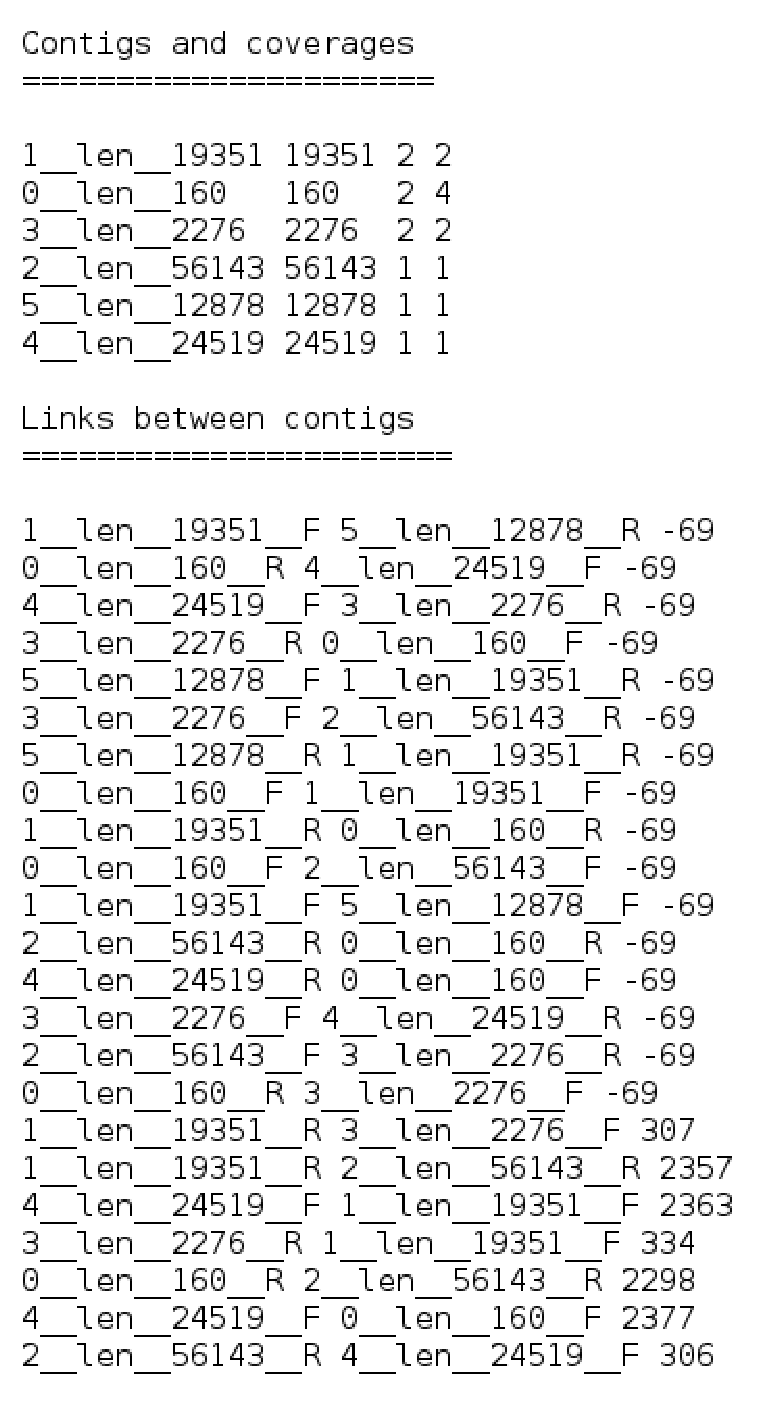
\includegraphics[scale=0.4]{agrostis_INPT_txt}};
\node (graph) at (11.5,0) {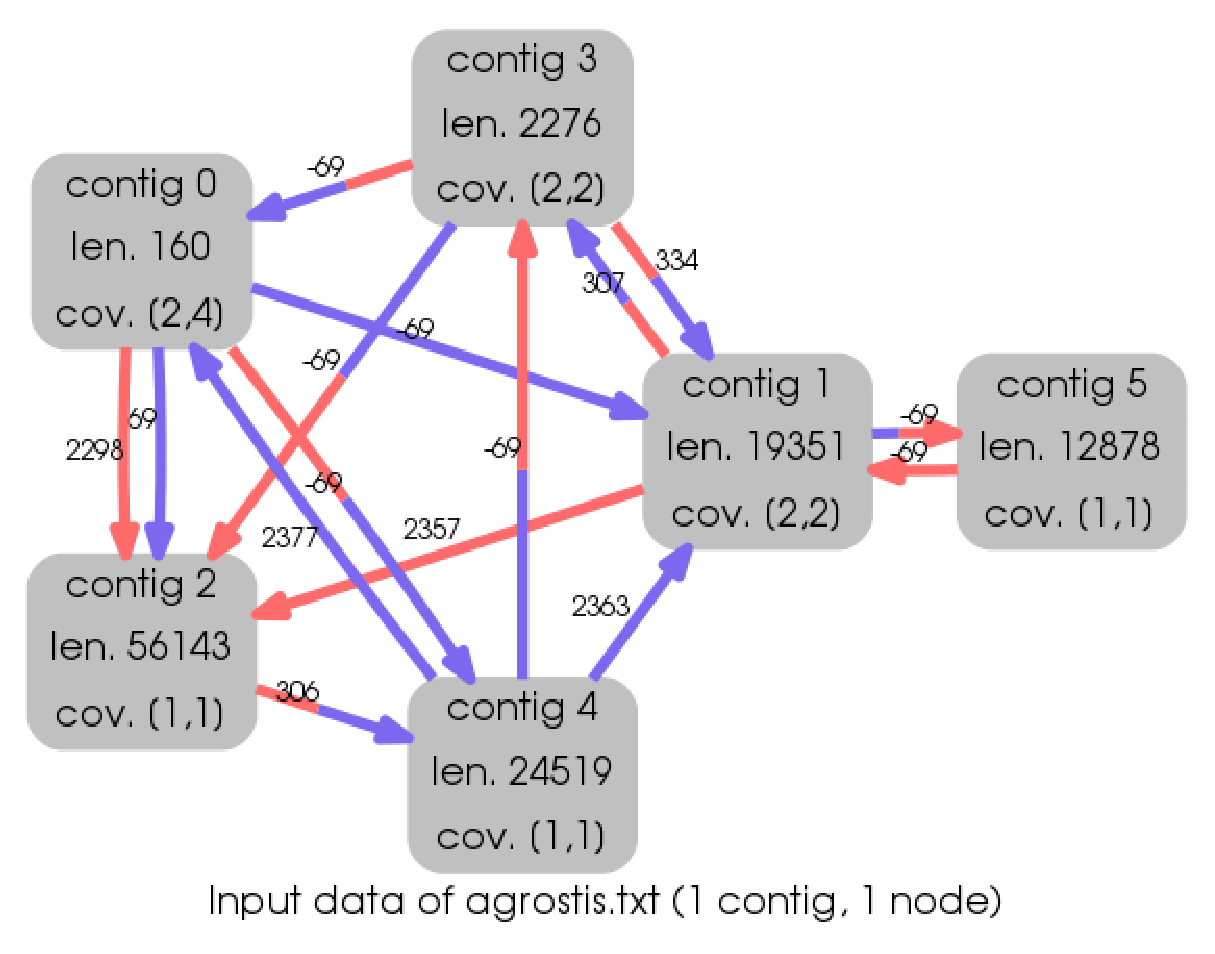
\includegraphics[scale=0.4]{agrostis_INPT_graph}};
\draw [line width=1mm, ->] (txt.east) -- (graph.west) node[midway, above] {\small \texttt{graph\_generator.py}};
\filldraw [color=red] (-2.6,0.4) circle (1.5pt);
\filldraw [color=red] (-2.6,-2.65) circle (1.5pt);
\end{tikzpicture}
}
\caption{Input data of \textit{Agrostis stolonifera} chloroplast genome in \textit{.txt} format and its graph representation}
\label{fig:inpagrostis}
\scriptsize The \textit{.txt} file contains a list of unitigs with their associated length and coverage. When the coverage is $>1$ the unitig is a repeated sequence. The advantage of using unitigs and not contigs is that the associated coverage is easier to determine (for long unitigs) and more trustworthy. For small unitigs, the coverage is an interval (here, the 160 base unitig 0). The joins between unitigs are orientated and contain the contig orientation (\textit{Forward} or \textit{Reverse}) information. The distance of each link is negative when two unitigs overlap or positive when two unitigs are separated by a gap. Positive distances (gaps) are obtained though mate-pair information. In the graph orientations are represented by color: red for \textit{Reverse} and blue for \textit{Forward}.
\end{figure}

\vspace{-0.2cm}
\textbf{How is the \textit{.txt} file obtained? }\\
The gaps (positive distance links) are obtained by mapping mate-paired reads on the unitigs as seen in figure \ref{fig:mappreads}. Overlaps are computed separately. GST are provided a ready list of links while most of the scaffolders (SSPACE, SOPRA \ldots) join construction is the first step of the scaffolder. Unitig coverage is obtained by mapping paired reads. The bigger the contig, the more robust the mapping information is - hence the intervals for small unitigs.

\newpage

\subsubsection{Features of the assembled genomes}
\label{sec:genomefeatures}
As the aim of the Genscale scaffolding project is to produce a complete genome rising to the challenge of repeated sequences, chloroplastic and bacterial genomes are well suited to test the performances of the GSTools. Moreover, chloroplastic and bacterial genomes are small enough to enable a detailed assessment and benchmarking of found solutions.

\textbf{Chloroplasts} \\
Chloroplasts are small organelles in plant photosynthetic tissues which possess their own DNA. The chloroplast genomes are small ($\approx 150kpb$), circular and have a large inverted repeated sequence of around $25kpb$. Some instances used in this study lack this repetition. This is the case in \textit{Pinus koraiensis} and \textit{Euglena gracilis}. However these two genomes possess significantly more small ($<$ 20bp) repeated sequences. 
\begin{figure}[h!]
\centering
\resizebox{1.7in}{!}{
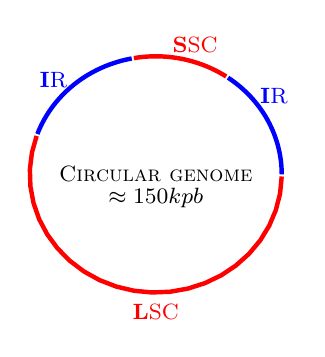
\begin{tikzpicture}
   \draw [blue,ultra thick,domain=0:55] plot ({1.6*cos(\x)}, {1.5*sin(\x)});
   \draw [red,ultra thick,domain=56:100] plot ({1.6*cos(\x)}, {1.5*sin(\x)});
   \draw [blue, ultra thick, domain=101:160] plot ({1.6*cos(\x)}, {1.5*sin(\x)});
   \draw [red, ultra thick, domain=161:359] plot ({1.6*cos(\x)}, {1.5*sin(\x)});
   \node[draw=none, fill=none] at (0,0) {\footnotesize \textsc{Circular genome }};
   \node[draw=none, fill=none] at (0,-0.3) {\footnotesize $\approx 150kpb$};
   \node[draw=none, fill=none] at (1.5,1) {\footnotesize \color{blue} \textbf IR};
   \node[draw=none, fill=none] at (-1.3,1.2) {\footnotesize \color{blue} \textbf IR};
   \node[draw=none, fill=none] at (0,-1.75) {\footnotesize \color{red} \textbf LSC};
   \node[draw=none, fill=none] at (0.5,1.65) {\footnotesize \color{red} \textbf SSC};
\end{tikzpicture}
}
\caption{Chloroplast genome structure}
{\footnotesize Inverted Repeat (IR $ \approx 23kpb$) ; Long Single Copy (LSC); Small Simple Copy (SSC $\approx 85kpb$)}
\end{figure} \\

\textbf{Bacteria and other} \\
Bacterial genomes are bigger ($>$ 1Mpb) and contain many small repeated sequences between 500pb and 1000pb.

\begin{figure}[h!]
\centering
\resizebox{15cm}{!}{
\begin{tikzpicture}
\node (1000) at (0,0) {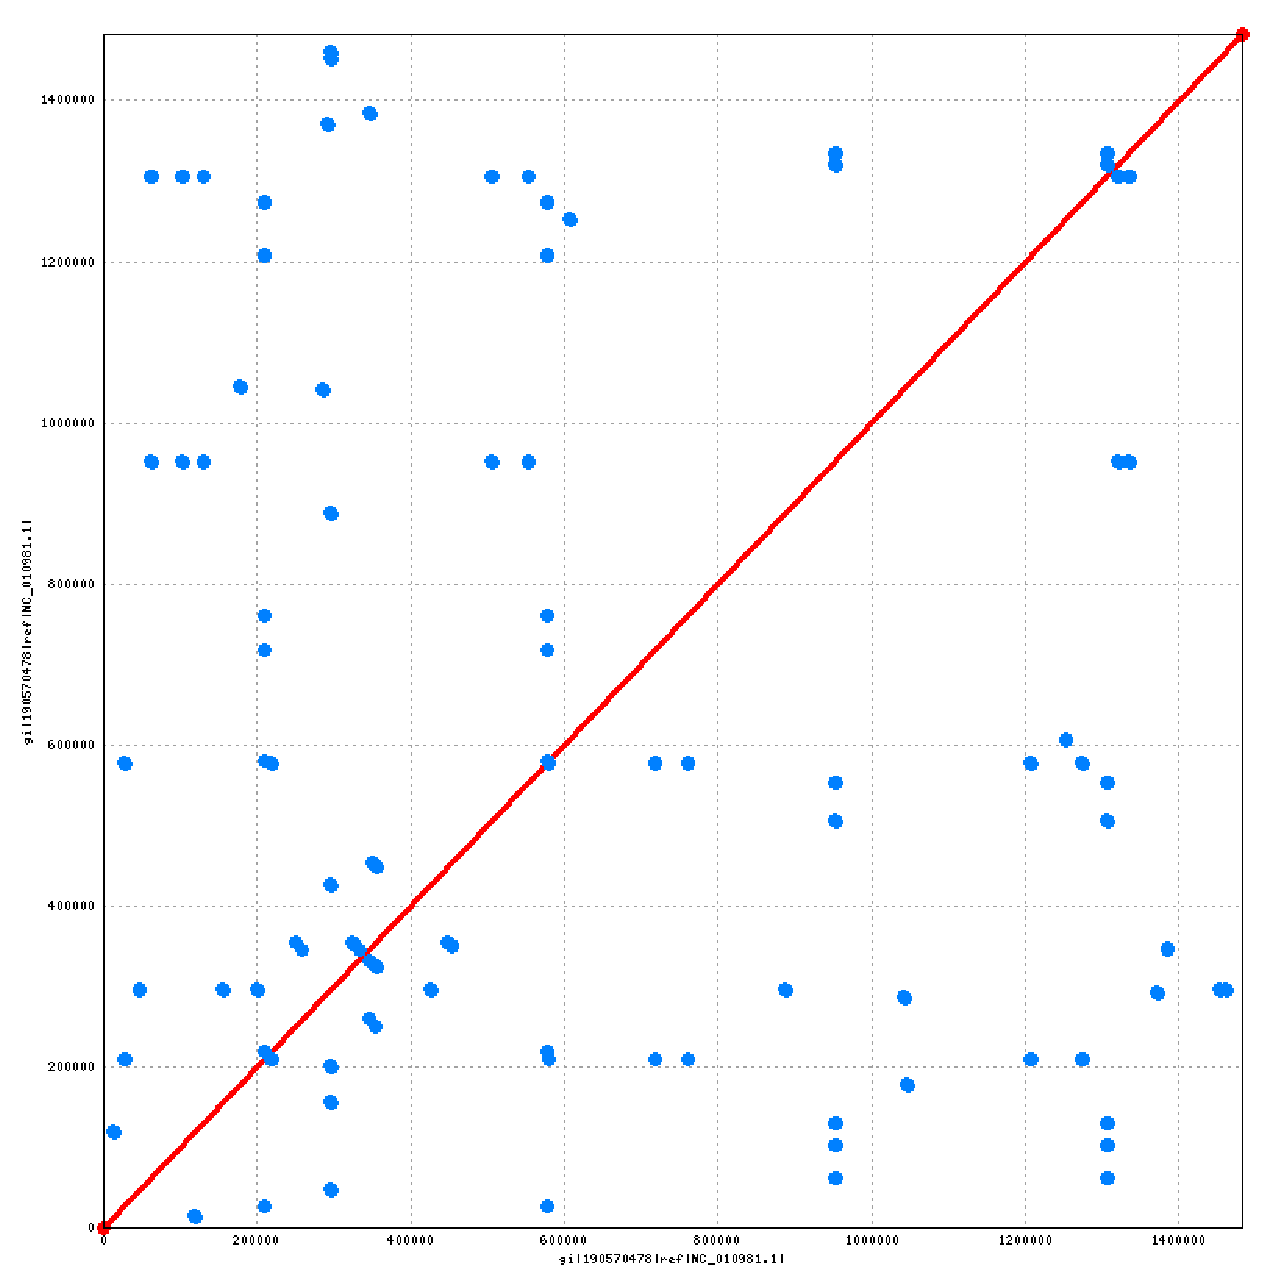
\includegraphics[scale=0.25]{wolba_vs_ref_1000}};
\node (500) at (6,0) {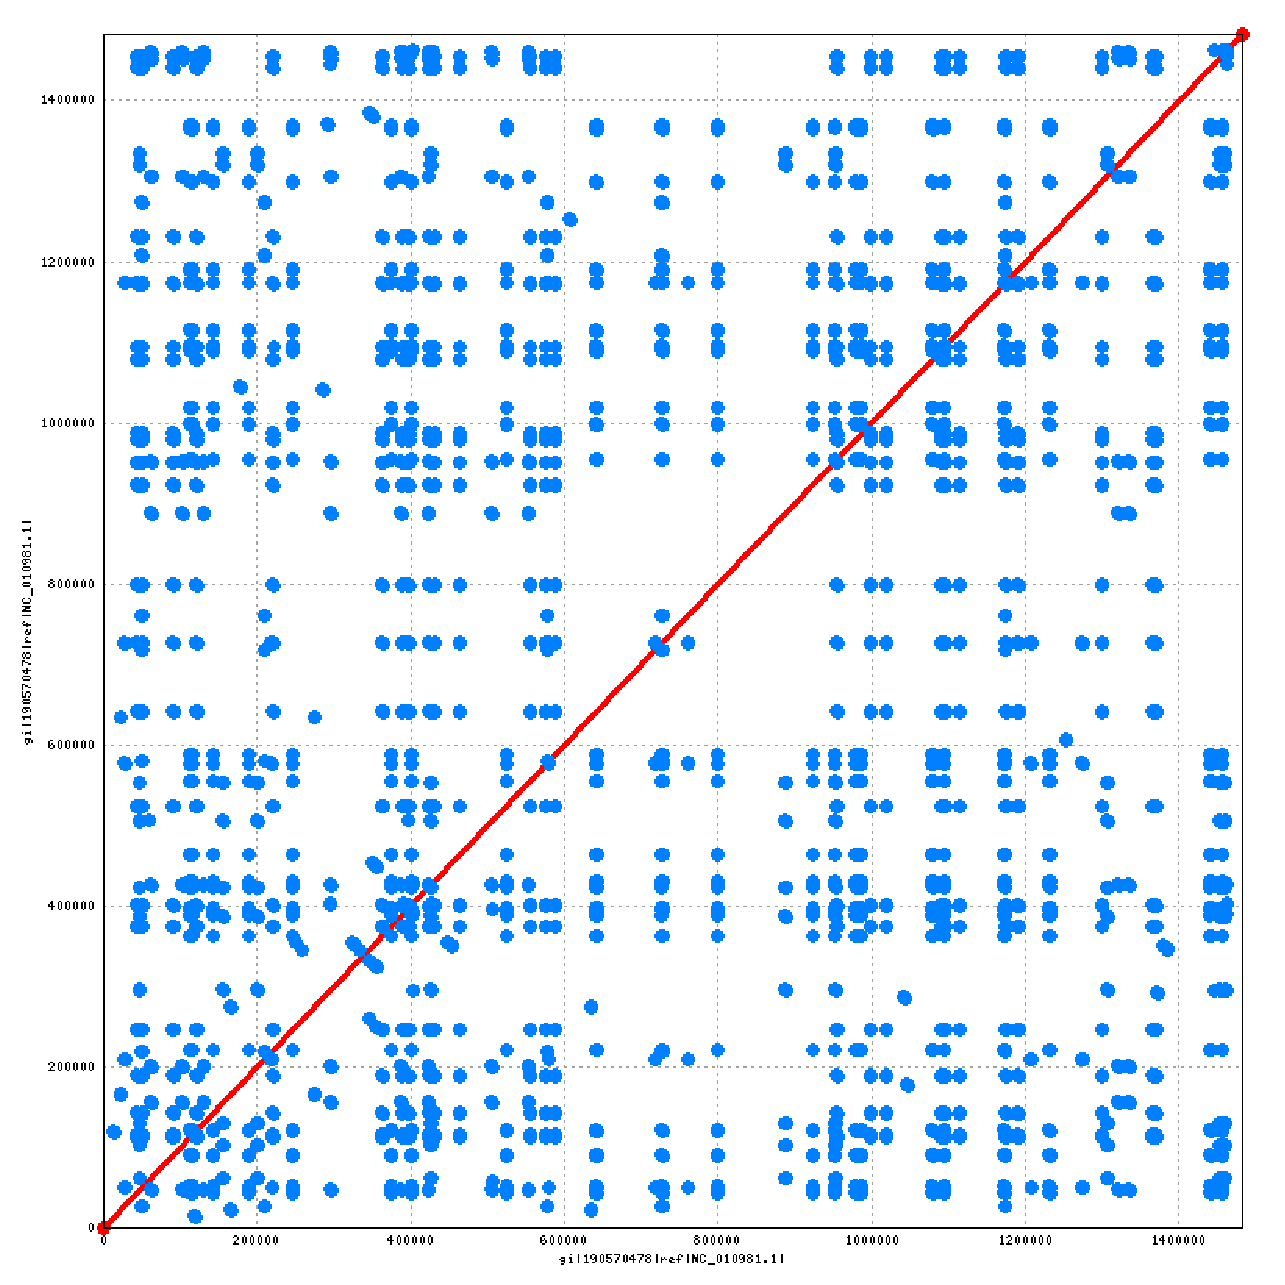
\includegraphics[scale=0.25]{wolba_vs_ref_500}};
\end{tikzpicture}
}
\caption{Wolbachia endosymbiont genome dotplotted against itself}
{\footnotesize Notes}
\label{fig:wolbarepeats}
\end{figure}

\newpage
\subsubsection{Genscale scaffolding strategies}
As seen in figure \ref{fig:inpagrostis}, the input data can be visualized by the \texttt{graph\_generator.py} script as a graph where nodes uniquely represent unitigs regardless of their coverage. However, this visualization is useful for a first human assessment of the data. Within models, each contig is multiplied by the number of occurrences. The total number of occurrences is then duplicated to model the \textit{Forward} and \textit{Reverse} orientation. With the number of contig occurrences and orientations, the number of links increases as well. However no duplicate links are allowed (merged) and for each link its reverse equivalent is created. A simple example of the difference between the raw input graph and the processed input graph that the GST solve is presented in figure \ref{fig:riceinpt}.

\begin{figure}[h!]
\centering
\resizebox{17cm}{!}{
\begin{tikzpicture}
\node (txt) at (0,0) {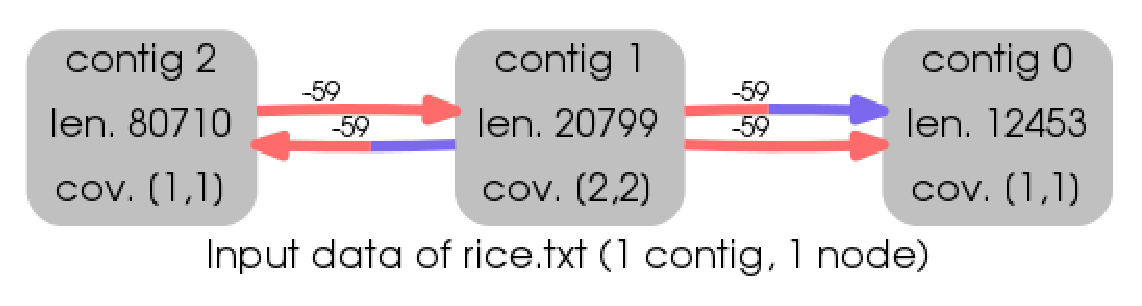
\includegraphics[scale=0.4]{rice_INPT_graph_G1}};
\node (graph) at (11,0) {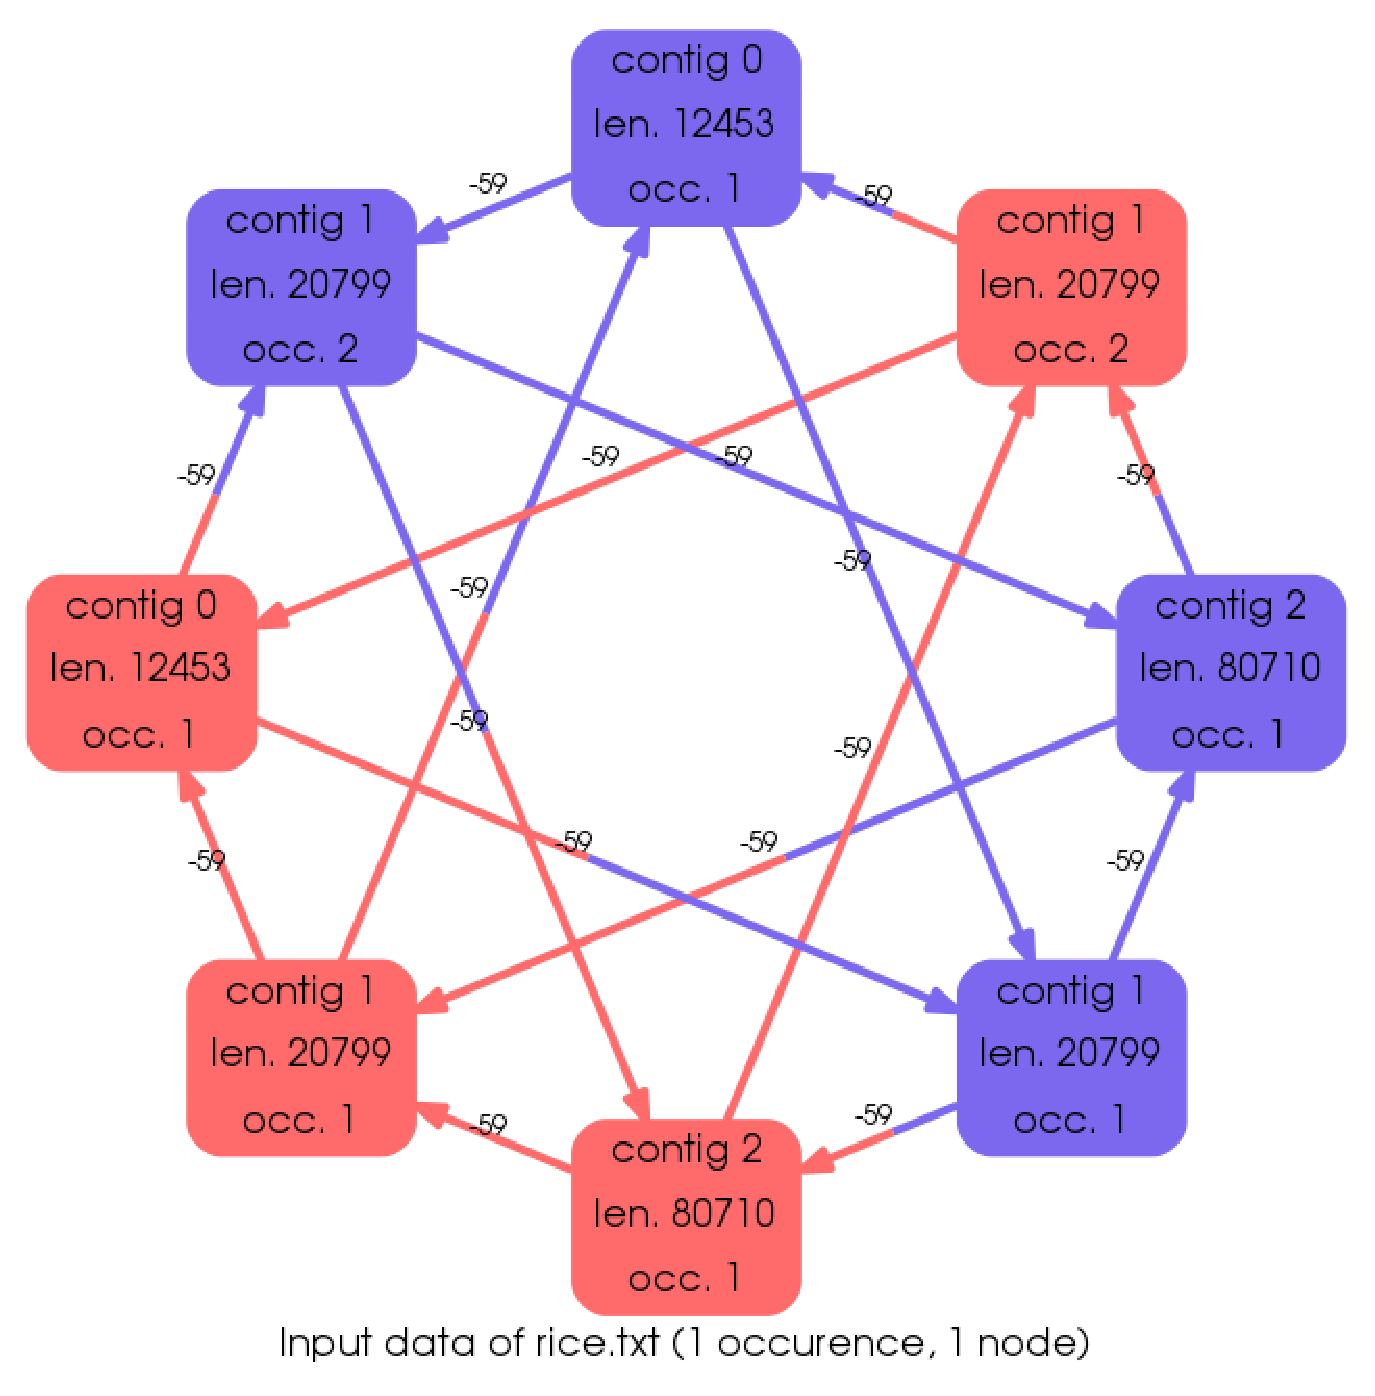
\includegraphics[scale=0.4]{rice_INPT_graph_G2}};
%\draw [line width=1mm, ->] (txt.east) -- (graph.west) node[midway, above] {\small \texttt{graph\_generator.py}};
\end{tikzpicture}
\caption{Input graphs of eucalyptus, as observed in the txt file and as processed by the Genscale scaffolding models}
\label{fig:riceinpt}
}
\end{figure}

%-------------------------------------------------------------------------------
% BODEH!
%-------------------------------------------------------------------------------
\subsection{Testing GST and search for the holy grail of explanations}
Golden standard et comparison between data etc

%-------------------------------------------------------------------------------
% BODEH!
%-------------------------------------------------------------------------------

\subsection{Benchmarking} \label{sec:benchmarking}
\subsubsection{Published scaffolders chosen for benchmarking}
Why i chose SSPACE?
\subsubsection{Benchmarking strategy}
\textbf{Draw a workflow}
Chosen scaffolding tools to benchmark against
Benchmarking workflow
Comparisons
QUAST
Comparison function
Visualization
MUMMER
Visualization tool
%-------------------------------------------------------------------------------
% BODEH!
%-------------------------------------------------------------------------------
\newpage
\section{Results}
\subsection{Comparison between the data sets}
\subsubsection{Input data sets}
Results presented in table \ref{tab:graphcomplexity} are those of the complete model-like graphs. 

\begin{table}[h!]
\resizebox{18cm}{!}{
\begin{tabular}{|l||c|c|c|c|c|c|c|}
\hline
organism & G type & G size & \#nodes & \#edges & node degree & betweeness centrality & degree centrality \\  
\hline
agrostis & chpl. &size& 22 & 106 & min 4, max 13, avg 9 & c4R, c4F, c1R & c2F, c2R, c4F\\
acineto & bacter &size& 924 & 9288 & min 0, max 183, avg 20 & c121F, c35R, c35F & c62R, c143R, c25R\\
acorus & chpl.&size& 30 & 204 & min 4, max 26, avg 13 & c5R, c1F, c3F & c5R, c3F, c3R\\
atropa & chpl.&size& 52 & 288 & min 3, max 19, avg 11 & c0R, c14F, c14R & c0R, c2R, c11R\\
cucumis & chpl.&size& 194 & 1790 & min 4, max 72, avg 18 & c17F, c17R, c47R & c17F, c17R, c26R\\
eucalyptus & chpl.&size& 8 & 16 & min 2, max 6, avg 4 & c2R, c1F, c0F & c2R, c1F, c0F\\
euglena & chpl.&size& 296 & 11894 & min 8, max 225, avg 80 & c24F, c26F, c24R & c24F, c36R, c36F\\
lecomtella & chpl.&size& 22 & 90 & min 2, max 17, avg 8 & c1R, c4R, c1F & c1R, c0R, c0F\\
oenothera & chpl.&size& 172 & 3222 & min 3, max 82, avg 37 & c9F, c13F, c-9R& c28R, c28F, c18R\\
pinus & chpl.&size& 122 & 658 & min 3, max 38, avg 10 & c0F, c1R, c0R & c0F, c1R, c0R\\
rice & chpl.&size& 8 & 16 & min 4, max 4, avg 4 & c2R, c0F, c1F & c2F, c1F, c1R\\
sacchar. & chr3 &size& 370 & 4416 & min 4, max 139, avg 23 & c45F, c58R, c21F & c21F, c58R, c18R\\
wolbachia & bacter &size& - & - & min -, max -, avg - & c-, c-, c- & c-, c-, c-\\
\hline
\end{tabular}
}
\caption{Graph complexity }
\label{tab:graphcomplexity}
\end{table}

\subsubsection{Input data inconsistencies detector}
\texttt{input\_inspector.py}



\newpage
\subsection{Comparison of GST solutions with the expected solution}
\begin{table}[h!]
\begin{center}
\resizebox{11cm}{!}{
\begin{tabular}{|l||c|c||c|c||l|}
\hline
organism & expected solution found & time & partial solution found & time & note\\
\hline
agrostis &-&-&-&-&- \\
acineto &-&-&-&-&- \\
acorus &-&-&-&-&- \\
atropa &-&-&-&-&- \\
cucumis &-&-&-&-&- \\
eucalyptus &-&-&-&-&- \\
euglena &-&-&-&-&- \\
lecomtella &-&-&-&-&- \\
oenothera &-&-&-&-&- \\
pinus &-&-&-&-&- \\
rice &-&-&-&-&- \\
sacchar. &-&-&-&-&- \\
wolbachia &-&-&-&-&- \\
\hline
\end{tabular}
}
\end{center}
\caption{Genscale scaffolders solutions}
\label{fig:solutions}
\end{table}

\subsubsection{Weighted path method}
\subsubsection{Distance based}
\subsubsection{Flow model}

\newpage
\subsection{Comparison between best GST solution and SSPACE}
\subsubsection{QUAST and comparison function}
Find similar table for rice, pinus and wolbachia in Annexes. 

\begin{table}[h!]
\begin{center}
\caption{All statistics are based on contigs of size $\geq$ 50 bp, unless otherwise noted (e.g., "\# contigs ($\geq$ 0 bp)" and "Total length ($\geq$ 0 bp)" include all contigs).}
\resizebox{18cm}{!}{
\begin{tabular}{|l*{7}{|r}|}
\hline
Assembly & wpm\_sol1.fsa & wpm\_sol2.fsa & wpm\_sol3.fsa & wpm\_sol4.fsa & dist\_sol & sspace\_sol & ref\_genome \\ \hline
\# contigs ($\geq$ 0 bp) & {\bf 1} & {\bf 1} & {\bf 1} & {\bf 1} & 2 & 3 & {\bf 1} \\ \hline
\# contigs ($\geq$ 1000 bp) & {\bf 1} & {\bf 1} & {\bf 1} & {\bf 1} & {\bf 1} & 2 & {\bf 1} \\ \hline
Total length ($\geq$ 0 bp) & 136584 & 136584 & 136584 & 136584 & {\bf 137641} & 115344 & 136584 \\ \hline
Total length ($\geq$ 1000 bp) & 136584 & 136584 & 136584 & 136584 & {\bf 137145} & 115184 & 136584 \\ \hline
\# contigs & {\bf 1} & {\bf 1} & {\bf 1} & {\bf 1} & {\bf 1} & 3 & {\bf 1} \\ \hline
Largest contig & 136584 & 136584 & 136584 & 136584 & {\bf 137145} & 102256 & 136584 \\ \hline
Total length & 136584 & 136584 & 136584 & 136584 & {\bf 137145} & 115344 & 136584 \\ \hline
Reference length & 136584 & 136584 & 136584 & 136584 & 136584 & 136584 & 136584 \\ \hline
GC (\%) & 38.45 & 38.45 & 38.45 & 38.45 & 38.45 & 37.39 & 38.45 \\ \hline
Reference GC (\%) & 38.45 & 38.45 & 38.45 & 38.45 & 38.45 & 38.45 & 38.45 \\ \hline
N50 & 136584 & 136584 & 136584 & 136584 & {\bf 137145} & 102256 & 136584 \\ \hline
NG50 & 136584 & 136584 & 136584 & 136584 & {\bf 137145} & 102256 & 136584 \\ \hline
N75 & 136584 & 136584 & 136584 & 136584 & {\bf 137145} & 102256 & 136584 \\ \hline
NG75 & 136584 & 136584 & 136584 & 136584 & {\bf 137145} & 12928 & 136584 \\ \hline
L50 & 1 & 1 & 1 & 1 & 1 & 1 & 1 \\ \hline
LG50 & 1 & 1 & 1 & 1 & 1 & 1 & 1 \\ \hline
L75 & 1 & 1 & 1 & 1 & 1 & 1 & 1 \\ \hline
LG75 & {\bf 1} & {\bf 1} & {\bf 1} & {\bf 1} & {\bf 1} & 2 & {\bf 1} \\ \hline
\# misassemblies & {\bf 0} & 2 & 1 & 1 & 2 & 1 & {\bf 0} \\ \hline
\# misassembled contigs & {\bf 0} & 1 & 1 & 1 & 1 & 1 & {\bf 0} \\ \hline
Misassembled contigs length & {\bf 0} & 136584 & 136584 & 136584 & 137145 & 102256 & {\bf 0} \\ \hline
\# local misassemblies & {\bf 0} & {\bf 0} & {\bf 0} & {\bf 0} & 1 & {\bf 0} & {\bf 0} \\ \hline
\# unaligned contigs & 0 + 0 part & 0 + 0 part & 0 + 0 part & 0 + 0 part & 0 + 0 part & 0 + 0 part & 0 + 0 part \\ \hline
Unaligned length & 0 & 0 & 0 & 0 & 0 & 0 & 0 \\ \hline
Genome fraction (\%) & {\bf 100.000} & {\bf 100.000} & 98.657 & 98.657 & 91.522 & 84.590 & {\bf 100.000} \\ \hline
Duplication ratio & 1.000 & 1.155 & 1.014 & 1.014 & 1.097 & {\bf 0.998} & 1.000 \\ \hline
\# N's per 100 kbp & {\bf 0.00} & {\bf 0.00} & {\bf 0.00} & {\bf 0.00} & 218.75 & 12.14 & {\bf 0.00} \\ \hline
\# mismatches per 100 kbp & 0.00 & 0.00 & 0.00 & 0.00 & 0.00 & 0.00 & 0.00 \\ \hline
\# indels per 100 kbp & {\bf 0.00} & {\bf 0.00} & {\bf 0.00} & {\bf 0.00} & 5.60 & 0.87 & {\bf 0.00} \\ \hline
\# genes & 132 + 1 part & {\bf 133 + 0 part} & 131 + 0 part & 131 + 0 part & 122 + 1 part & 114 + 2 part & {\bf 133 + 0 part} \\ \hline
Largest alignment & {\bf 136584} & 81612 & 82913 & 134750 & 102364 & 81140 & {\bf 136584} \\ \hline
NA50 & {\bf 136584} & 81612 & 82913 & 134750 & 102364 & 81140 & {\bf 136584} \\ \hline
NGA50 & {\bf 136584} & 81612 & 82913 & 134750 & 102364 & 81140 & {\bf 136584} \\ \hline
NA75 & {\bf 136584} & 53138 & 53671 & 134750 & 22817 & 21116 & {\bf 136584} \\ \hline
NGA75 & {\bf 136584} & 53138 & 53671 & 134750 & 22817 & 12928 & {\bf 136584} \\ \hline
LA50 & 1 & 1 & 1 & 1 & 1 & 1 & 1 \\ \hline
LGA50 & 1 & 1 & 1 & 1 & 1 & 1 & 1 \\ \hline
LA75 & {\bf 1} & 2 & 2 & {\bf 1} & 2 & 2 & {\bf 1} \\ \hline
LGA75 & {\bf 1} & 2 & 2 & {\bf 1} & 2 & 3 & {\bf 1} \\ \hline
\end{tabular}
}
\end{center}
\end{table}

\begin{table}[h!]
\scriptsize
\begin{center}
\caption{All statistics are based on contigs of size $\geq$ 50 bp, unless otherwise noted (e.g., "\# contigs ($\geq$ 0 bp)" and "Total length ($\geq$ 0 bp)" include all contigs).}
\resizebox{10cm}{!}{
\begin{tabular}{|l*{4}{|r}|}
\hline
Assembly & wpm\_sol1.fsa & sspace\_sol & flow\_step1\_sol & ref\_genome \\ \hline
\# contigs ($\geq$ 0 bp) & {\bf 1} & 21 & 2 & {\bf 1} \\ \hline
\# contigs ($\geq$ 1000 bp) & 1 & 1 & 1 & 1 \\ \hline
Total length ($\geq$ 0 bp) & 116866 & {\bf 119654} & 116214 & 116866 \\ \hline
Total length ($\geq$ 1000 bp) & 116866 & {\bf 117042} & 115838 & 116866 \\ \hline
\# contigs & {\bf 1} & 21 & {\bf 1} & {\bf 1} \\ \hline
Largest contig & 116866 & {\bf 117042} & 115838 & 116866 \\ \hline
Total length & 116866 & {\bf 119654} & 115838 & 116866 \\ \hline
Reference length & 116866 & 116866 & 116866 & 116866 \\ \hline
GC (\%) & 38.80 & 38.83 & 38.86 & 38.80 \\ \hline
Reference GC (\%) & 38.80 & 38.80 & 38.80 & 38.80 \\ \hline
N50 & 116866 & {\bf 117042} & 115838 & 116866 \\ \hline
NG50 & 116866 & {\bf 117042} & 115838 & 116866 \\ \hline
N75 & 116866 & {\bf 117042} & 115838 & 116866 \\ \hline
NG75 & 116866 & {\bf 117042} & 115838 & 116866 \\ \hline
L50 & 1 & 1 & 1 & 1 \\ \hline
LG50 & 1 & 1 & 1 & 1 \\ \hline
L75 & 1 & 1 & 1 & 1 \\ \hline
LG75 & 1 & 1 & 1 & 1 \\ \hline
\# misassemblies & 11 & 2 & 1 & {\bf 0} \\ \hline
\# misassembled contigs & 1 & 1 & 1 & {\bf 0} \\ \hline
Misassembled contigs length & 116866 & 117042 & 115838 & {\bf 0} \\ \hline
\# local misassemblies & 4 & 5 & 4 & {\bf 0} \\ \hline
\# unaligned contigs & 0 + 0 part & 0 + 0 part & 0 + 0 part & 0 + 0 part \\ \hline
Unaligned length & 0 & 0 & 0 & 0 \\ \hline
Genome fraction (\%) & 99.471 & 99.892 & 92.153 & {\bf 100.000} \\ \hline
Duplication ratio & 1.005 & 1.025 & 1.076 & {\bf 1.000} \\ \hline
\# N's per 100 kbp & {\bf 0.00} & 741.30 & 6997.70 & {\bf 0.00} \\ \hline
\# mismatches per 100 kbp & 5.16 & 0.86 & {\bf 0.00} & {\bf 0.00} \\ \hline
\# indels per 100 kbp & 8.60 & 2.57 & 1.86 & {\bf 0.00} \\ \hline
\# genes & 262 + 7 part & 262 + 8 part & 249 + 4 part & {\bf 270 + 0 part} \\ \hline
Largest alignment & 28559 & 86569 & 96535 & {\bf 116866} \\ \hline
NA50 & 20762 & 86569 & 96535 & {\bf 116866} \\ \hline
NGA50 & 20762 & 86569 & 96535 & {\bf 116866} \\ \hline
NA75 & 19567 & 29474 & 96535 & {\bf 116866} \\ \hline
NGA75 & 19567 & 29474 & 96535 & {\bf 116866} \\ \hline
LA50 & 3 & {\bf 1} & {\bf 1} & {\bf 1} \\ \hline
LGA50 & 3 & {\bf 1} & {\bf 1} & {\bf 1} \\ \hline
LA75 & 4 & 2 & {\bf 1} & {\bf 1} \\ \hline
LGA75 & 4 & 2 & {\bf 1} & {\bf 1} \\ \hline
\end{tabular}
}
\end{center}
\end{table}
\newpage

\subsubsection{Visualization with mummer and graph\_generator.py}
\paragraph{graph\_generator.py visualization}
\hspace*{1cm}
\begin{figure}[h!]
\begin{center}
\resizebox{18cm}{!}{
\begin{tikzpicture}
\node (wpm1) at (0,0) {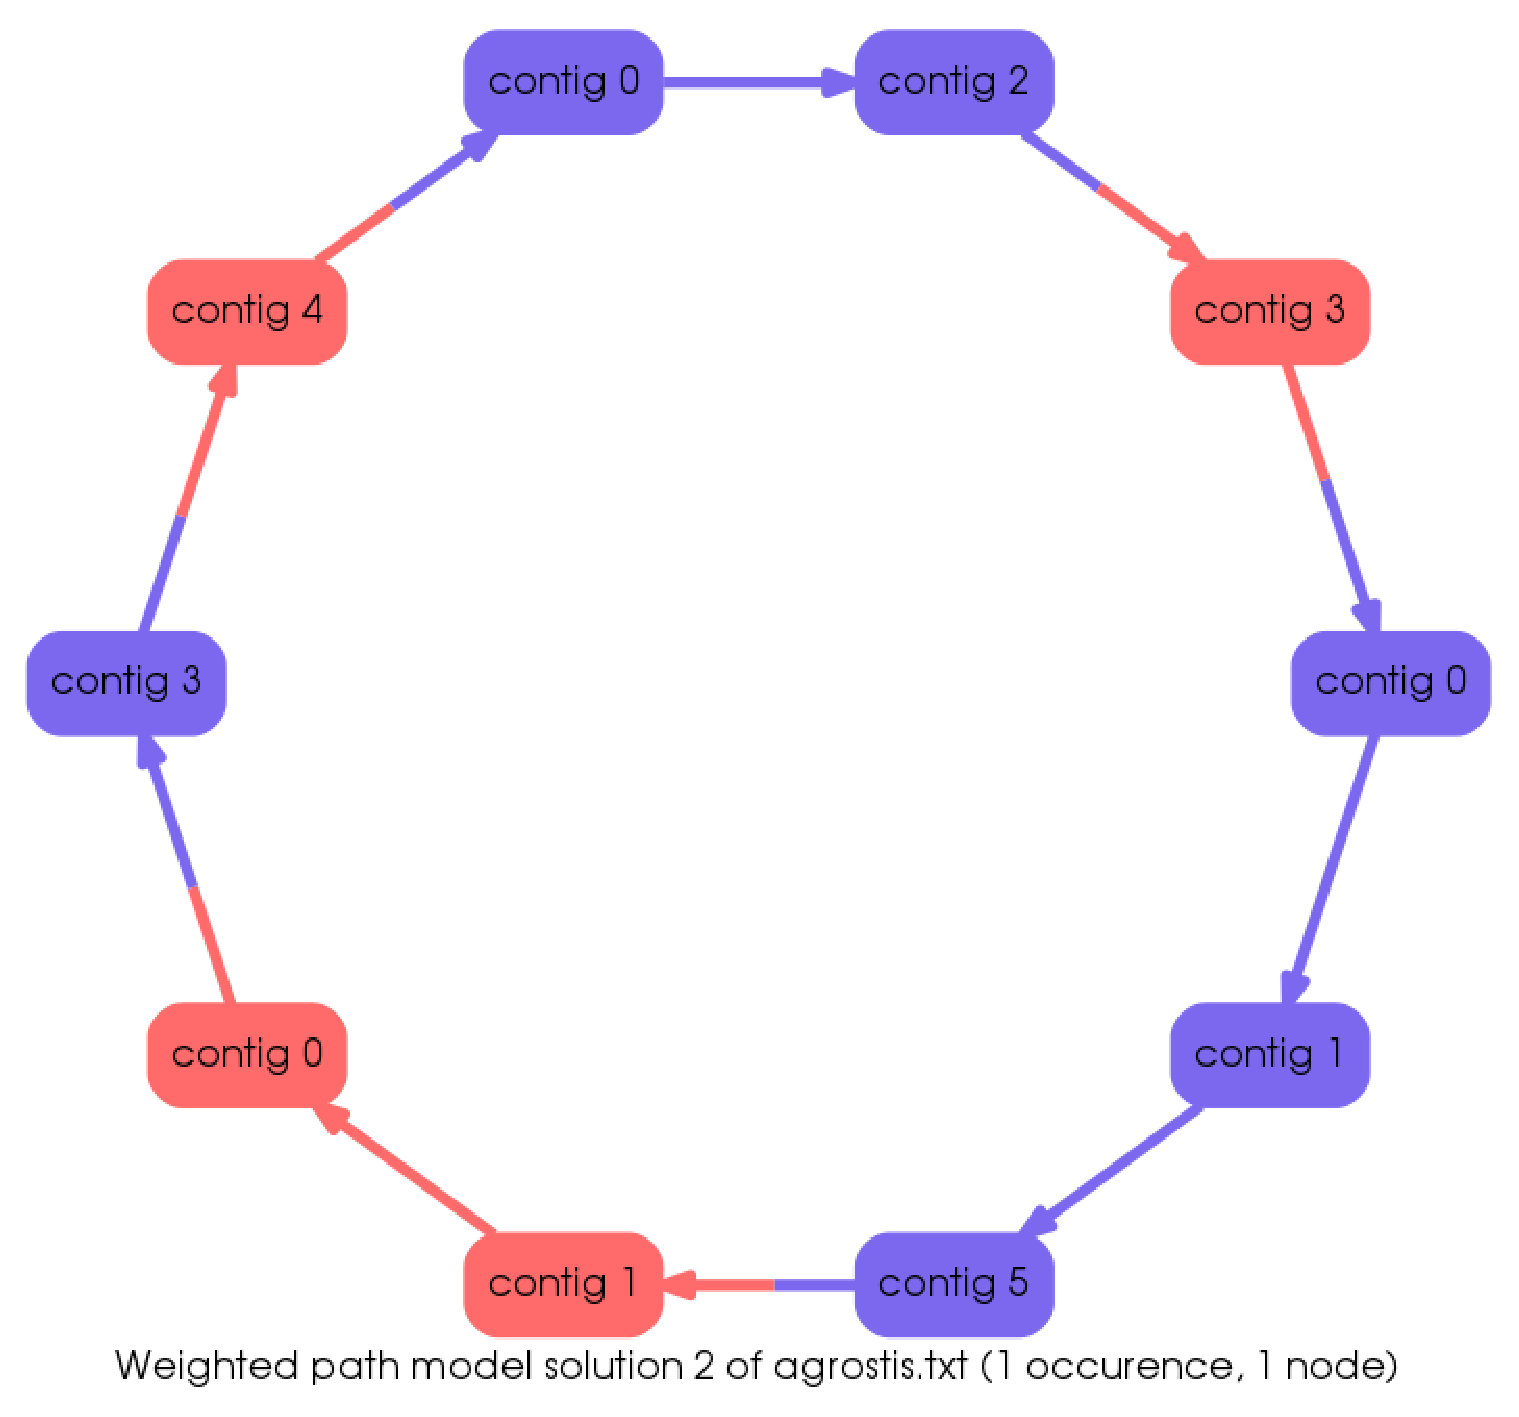
\includegraphics[scale=0.25]{wpm_agrostis_sol1}};
\node (wmp2) at (8,0) {\includegraphics[scale=0.25]{wpm_agrosti_sol2}};
\node (sspace) at (9,7) {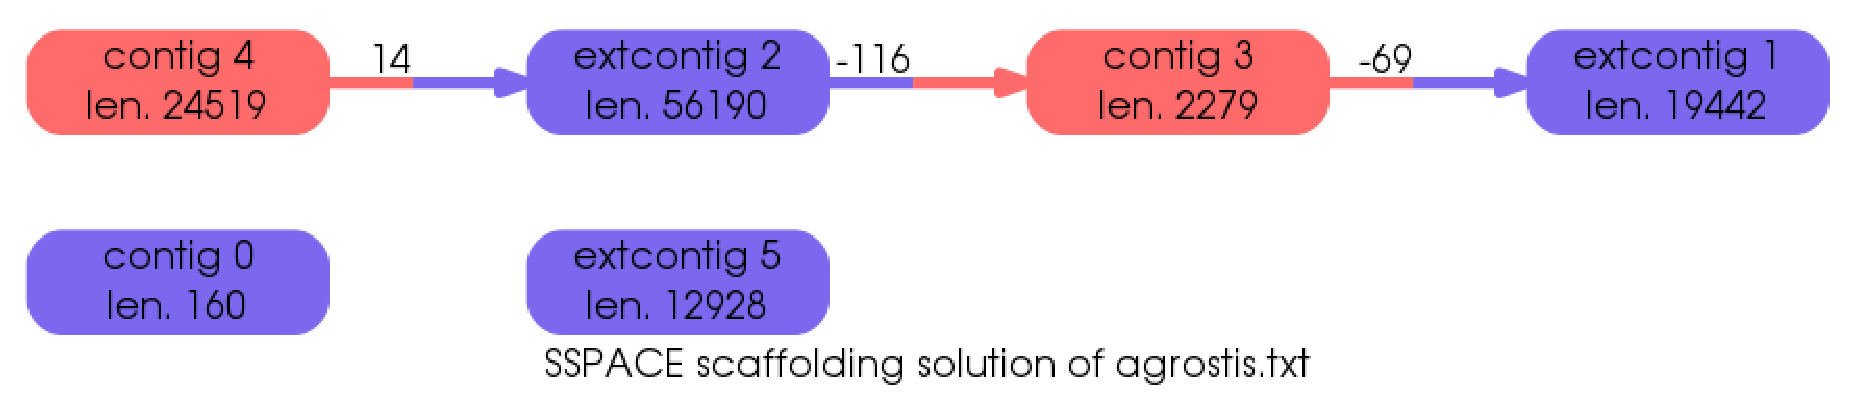
\includegraphics[scale=0.25]{sspace_scaffolds_agrostis}};
\node (gold) at (0,7) {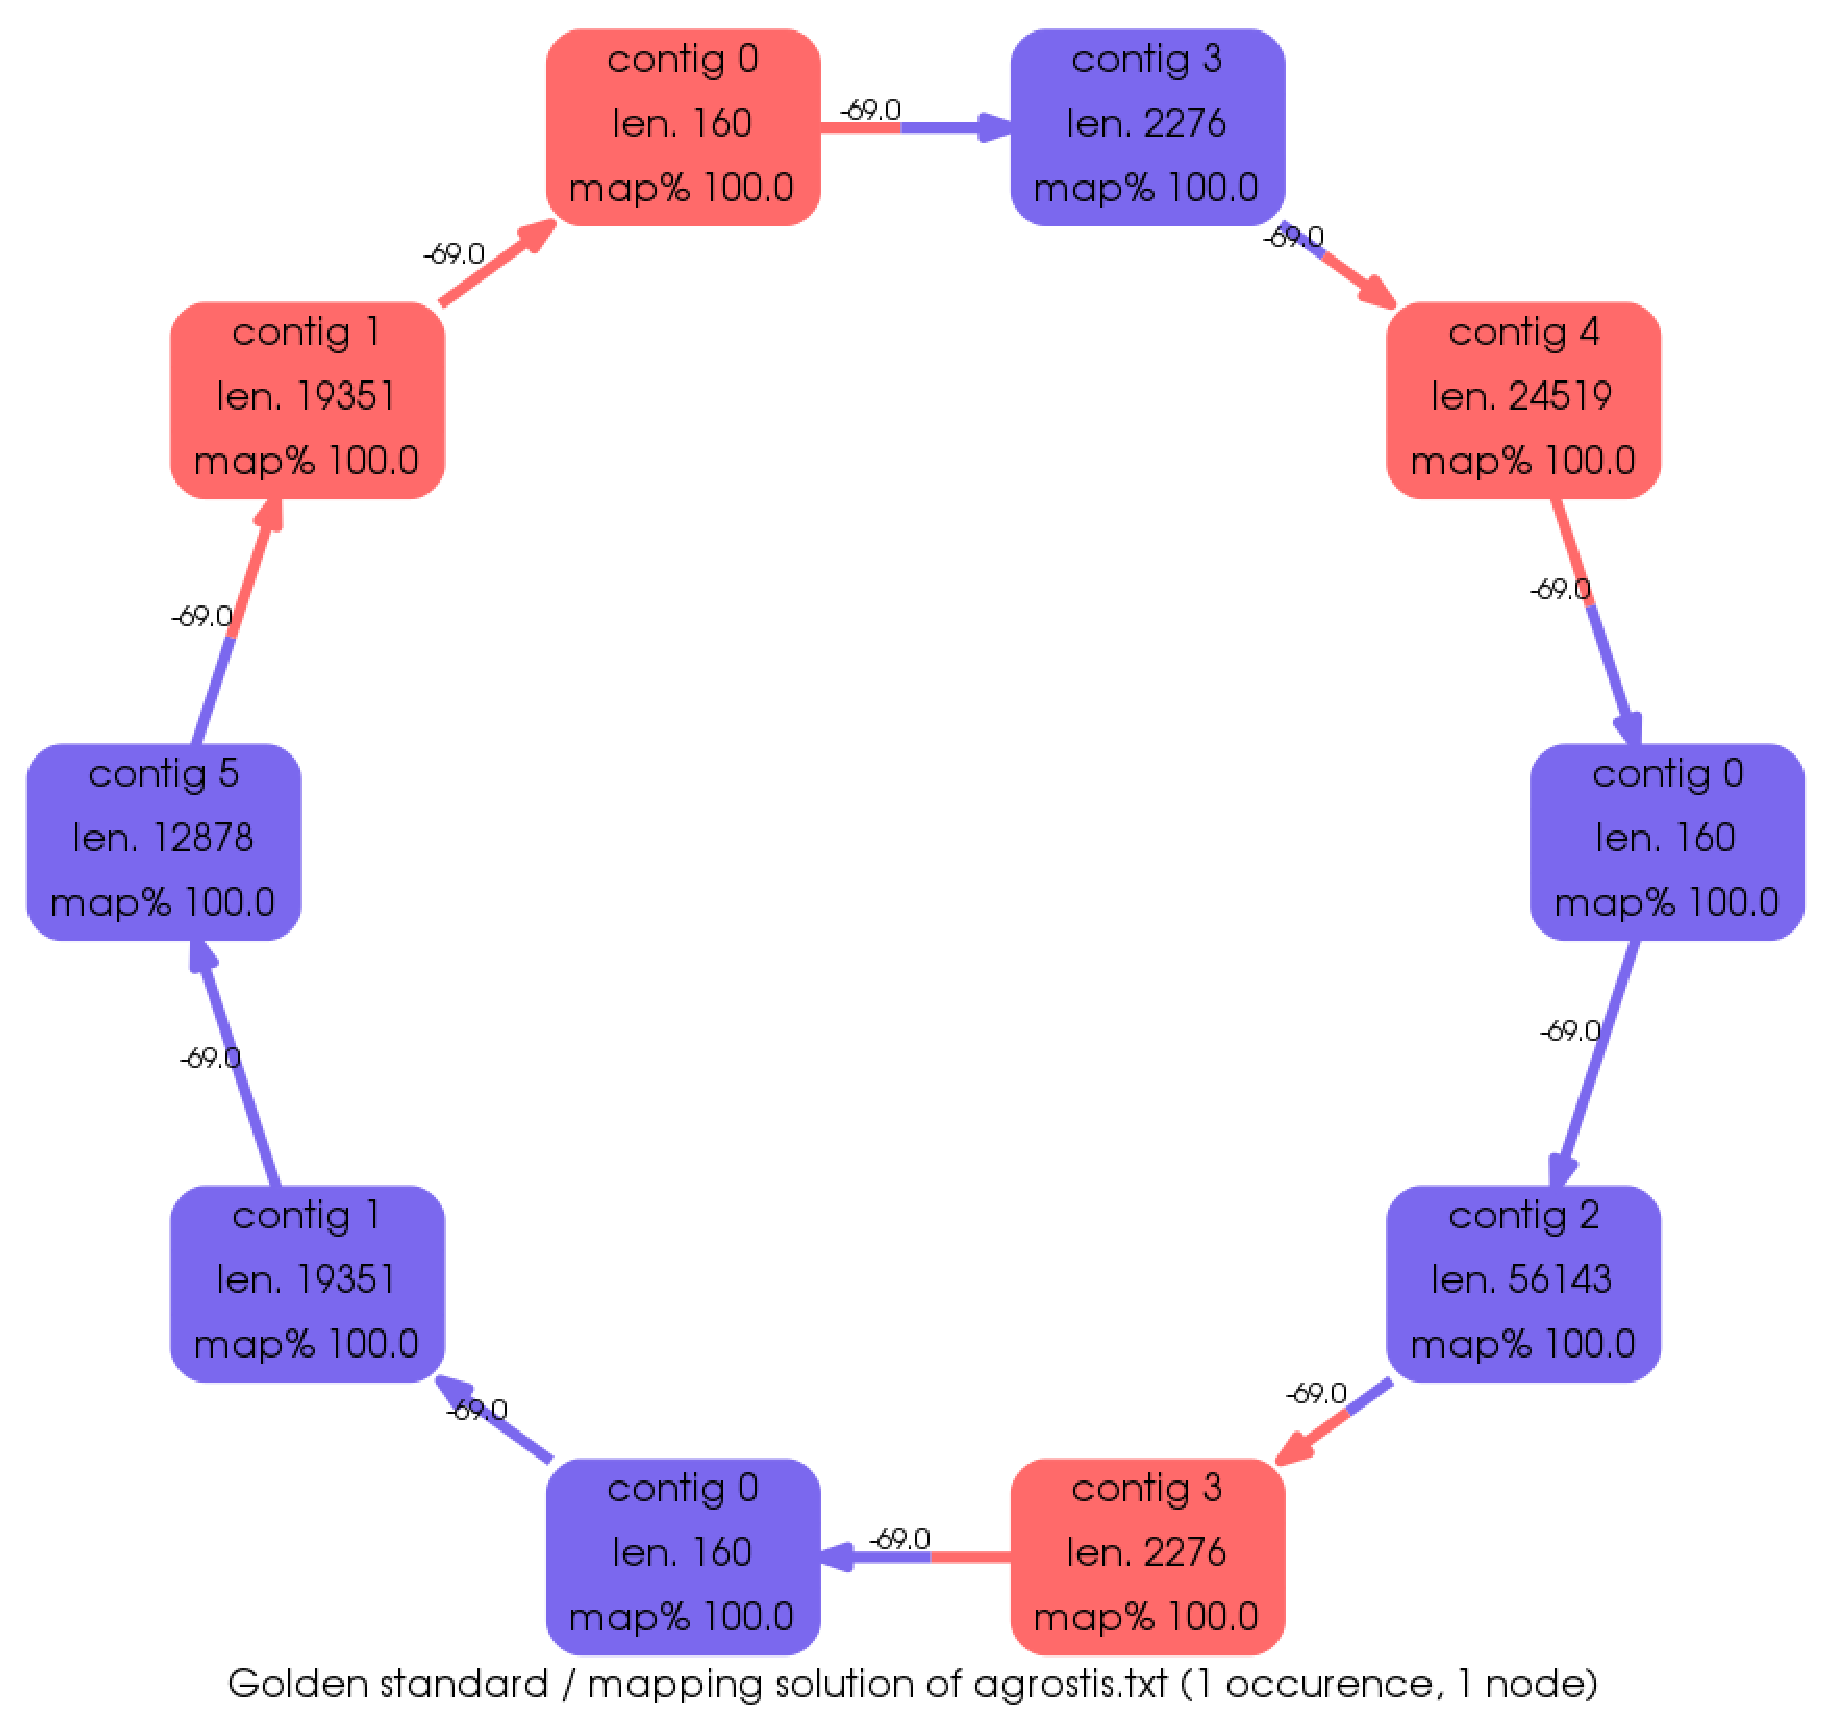
\includegraphics[scale=0.25]{agrostis_GOLD}};
\end{tikzpicture}
}
\end{center}
\caption{Expected solution and scaffolding solutions of weighted-path model and SSPACE scaffolders}
\label{scafsols}
\end{figure}
\newpage

\paragraph{Dotplots with mummer}
\hspace*{1cm}
\begin{figure}[h!]
\begin{center}
\resizebox{18cm}{!}{
\begin{tikzpicture}
\node (wpm1) at (0,-7) {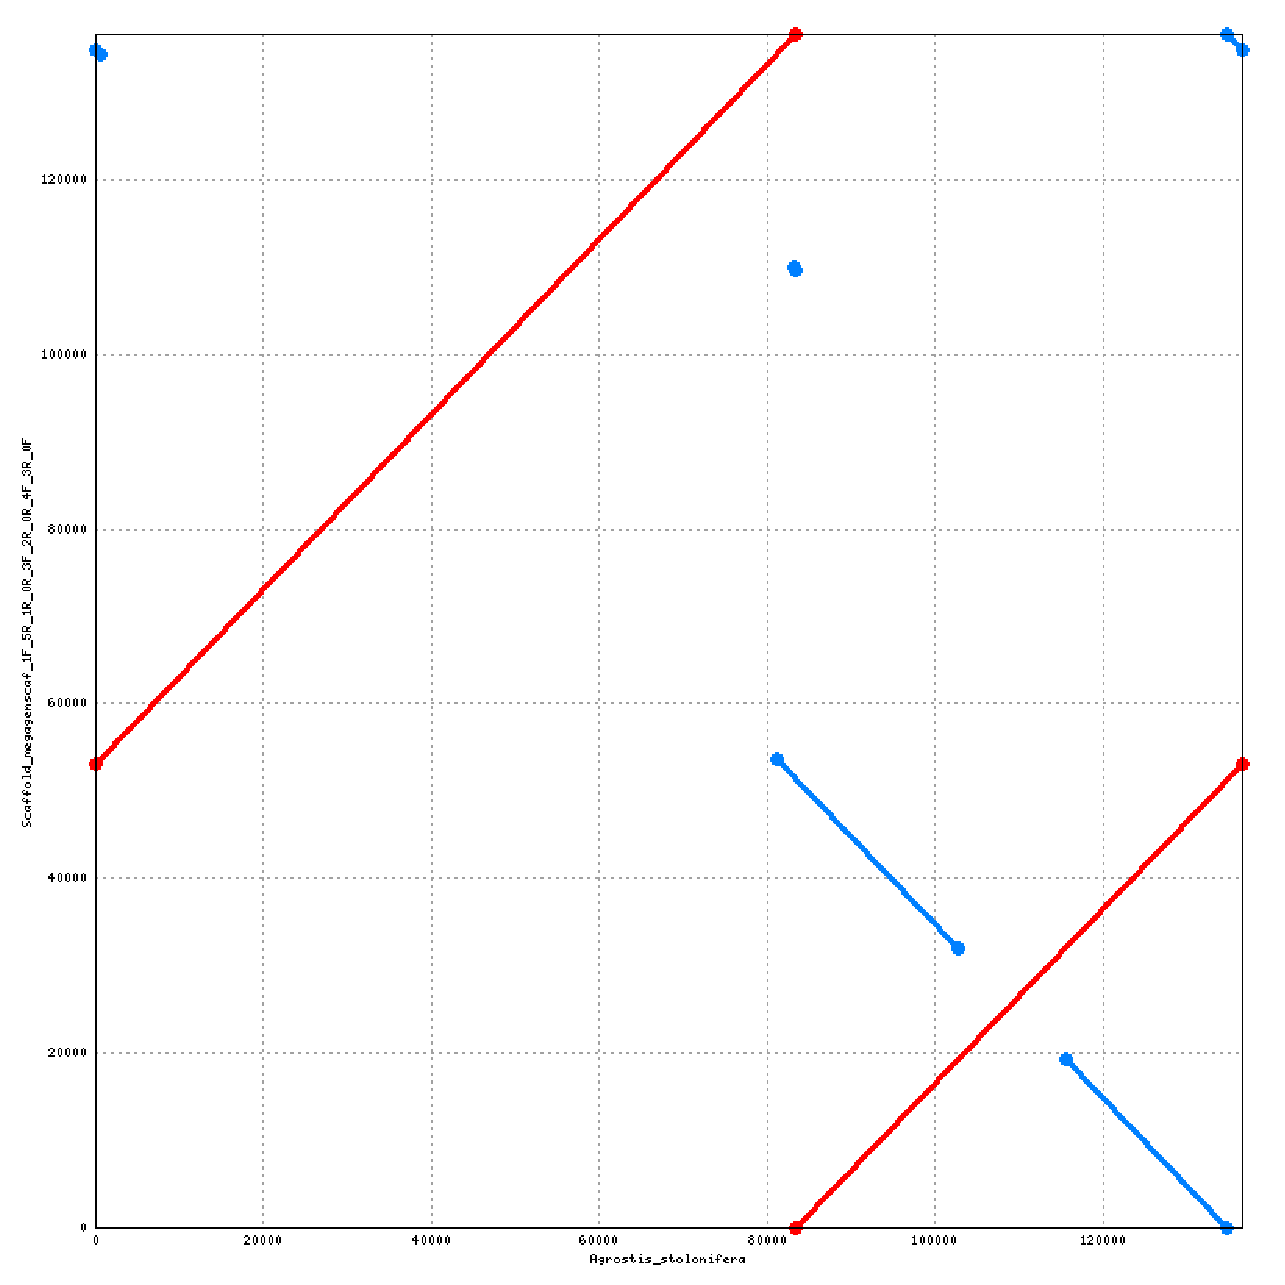
\includegraphics[scale=0.3]{dotplot_agro_wpm1}};
\node (wmp2) at (8,-7) {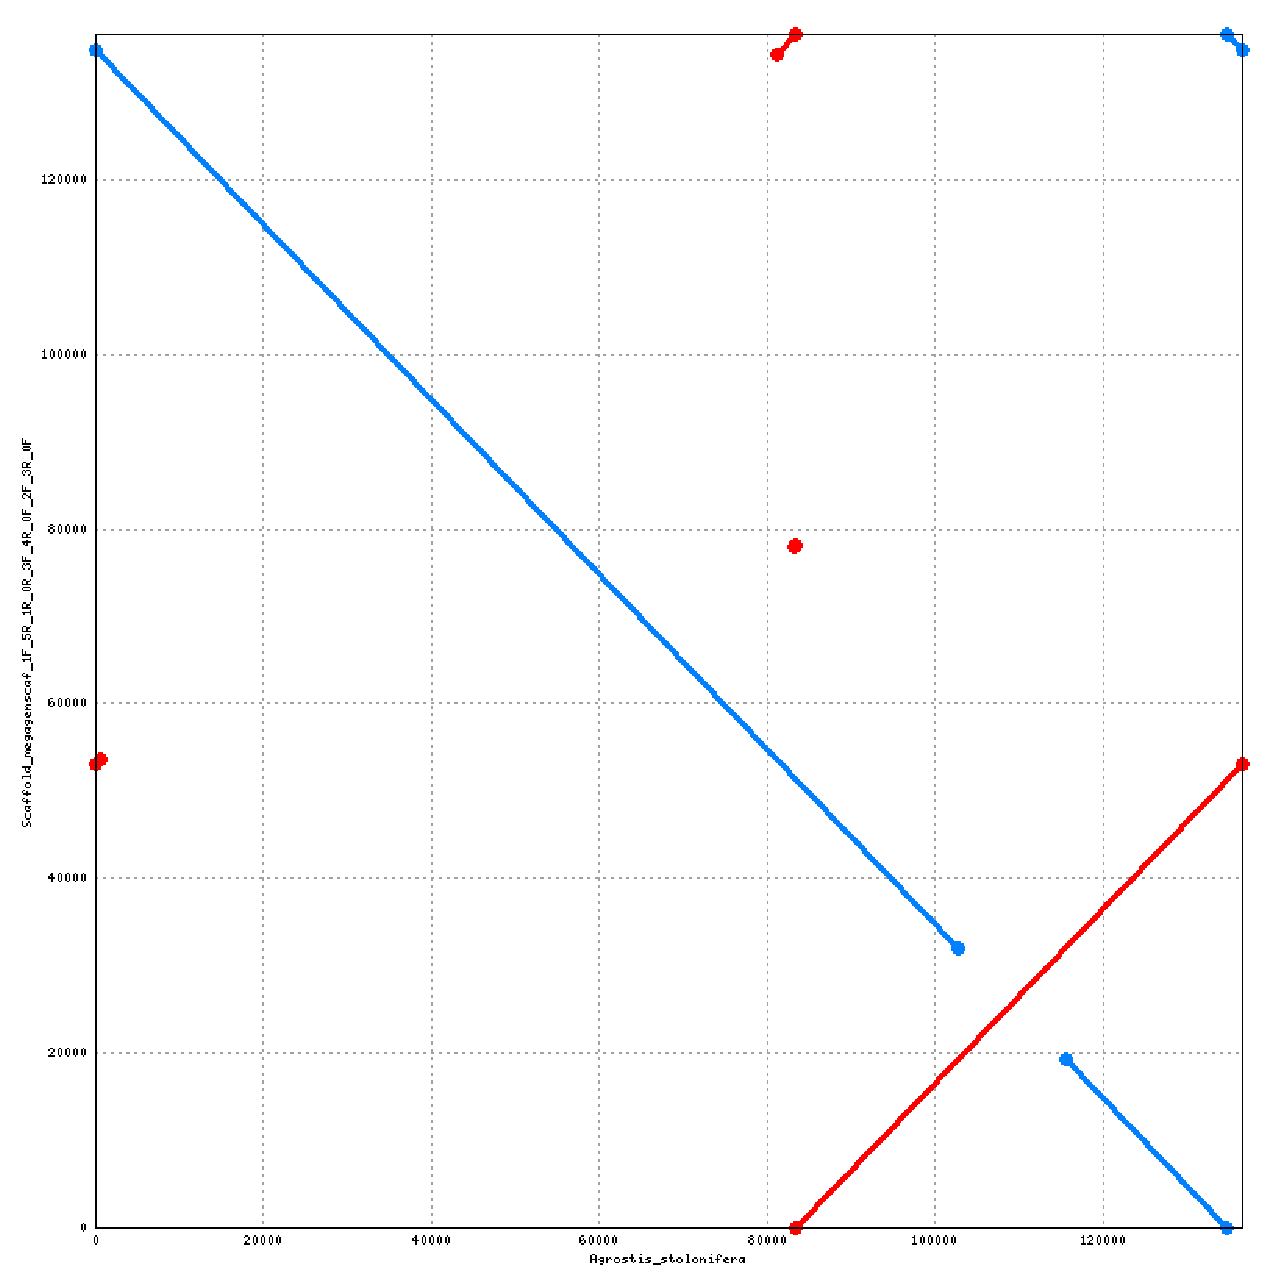
\includegraphics[scale=0.3]{dotplot_agro_wpm2}};
\node (ref) at (8,0) {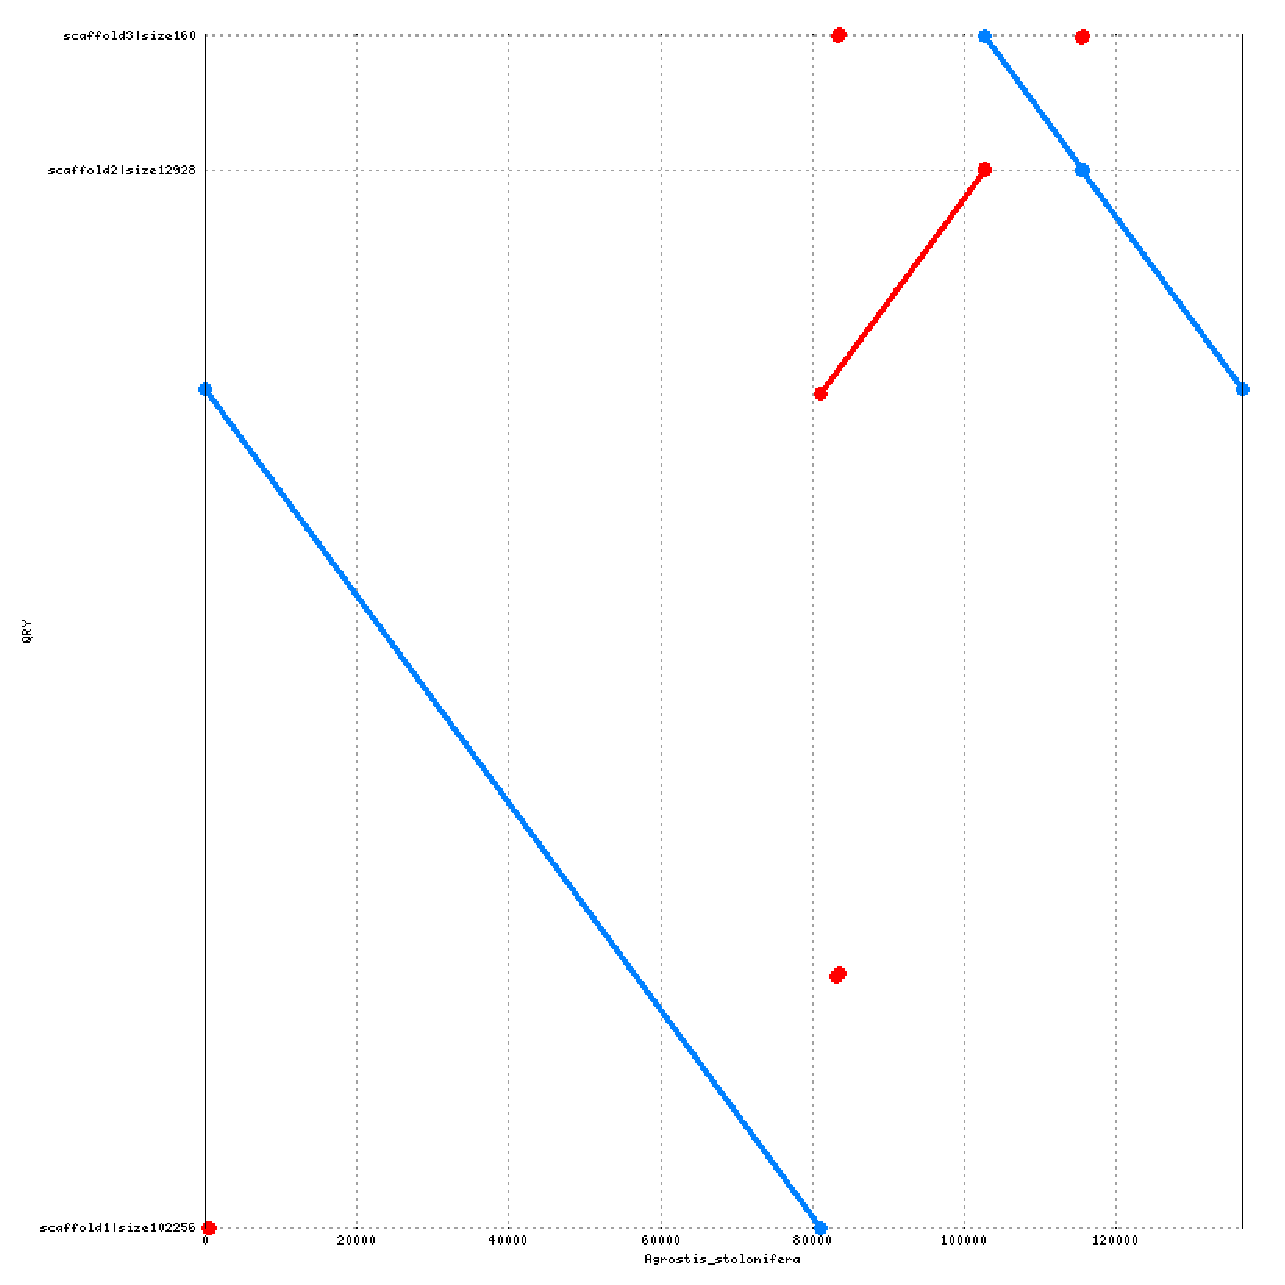
\includegraphics[scale=0.3]{dotplot_agro_sspace}};
\node (sspace) at (0,0) {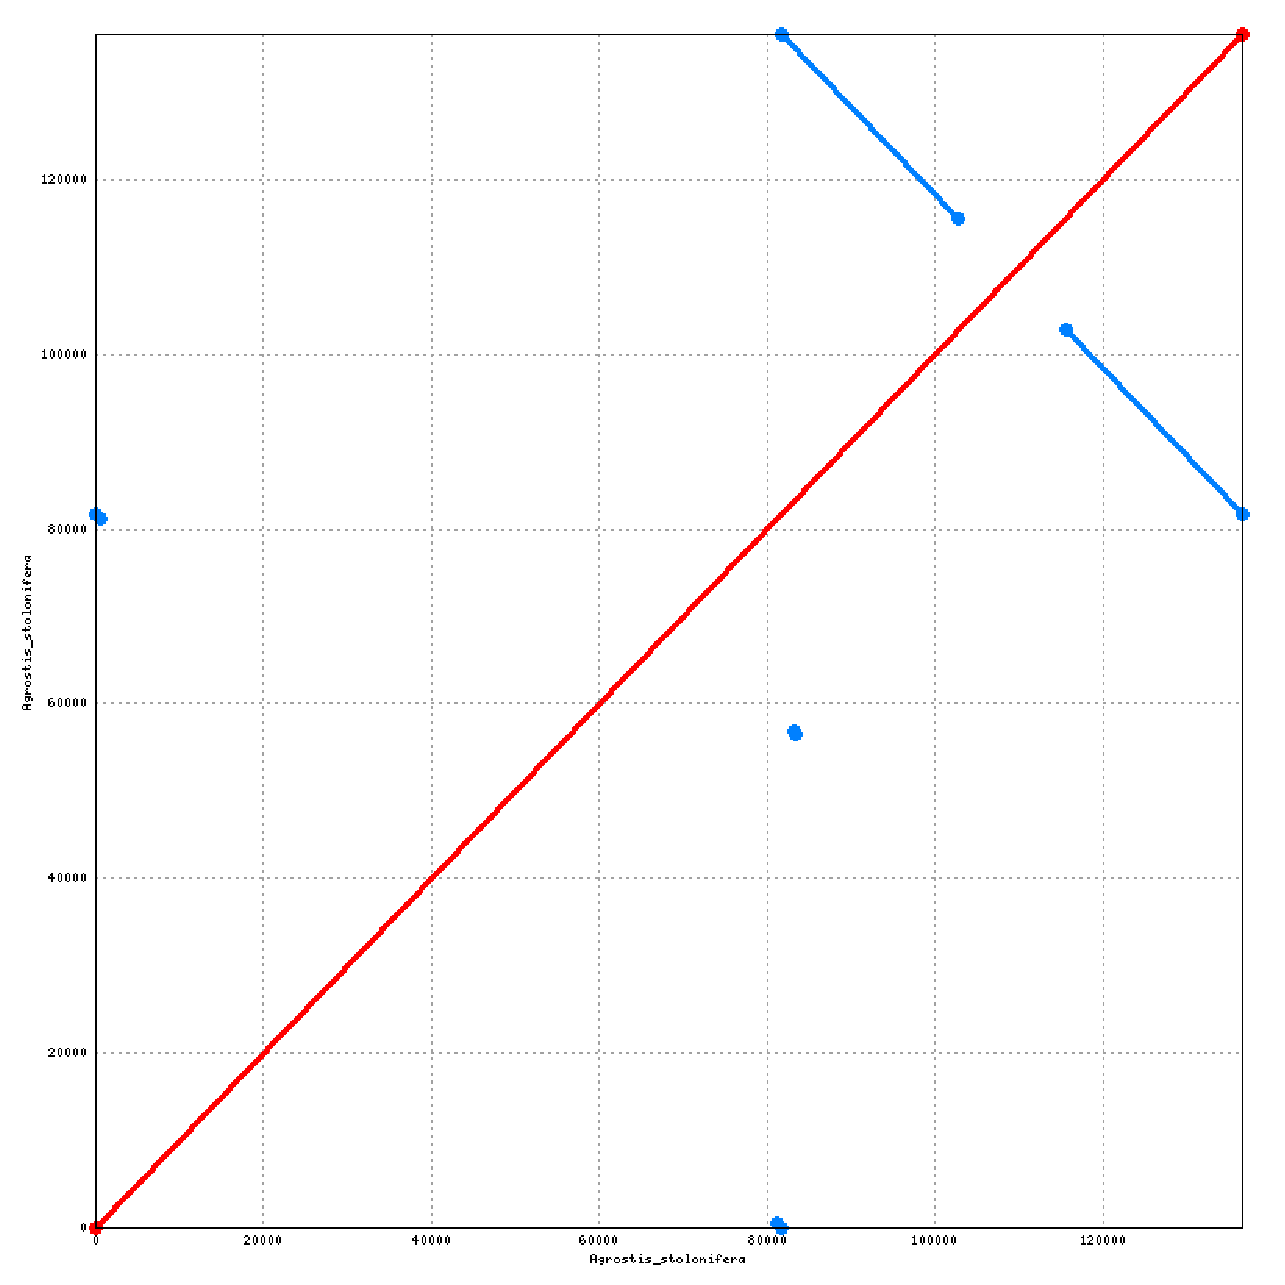
\includegraphics[scale=0.3]{dotplot_agrostis_agrostis}};
\end{tikzpicture}
}
\end{center}
\caption{Control dotplot and dotplots of weighted path model and SSPACE scaffolding solution with the reference genome}
\label{dotplotsols}
\end{figure}


\clearpage
\subsection{Partially solved instances}
The bacterial genomes are partially assembled by the flow model, which processes big mate-pair connected unitigs first. The wolbachia example highlights the importance of correctly choosing the mate pairs' insert size. The results presented in table \ref{tab:insert} show a drastic improvement of the total assembled length when changing the mate paired insert size from 1000bp to 2000bp. This length gradually decreases as the insert size increases (same with the genome size metric). The largest scaffold is also assembled with the 2000bp library (over 2000bp whereas all other libraries yield scaffolds $<$ 500kb). One proposed explanation is the repeats' sequence size of \textit{Wolbachia Endosymbiont}. As previously seen in \fulleref{fig:wolbarepeats} section \fullref{sec:genomefeatures} \nameref{sec:genomefeatures}, the bacterial genome has repeats with sizes mainly between 500bp and 1kbp. These repeats are partially solved during the unitig building step. The issue comes from genomically close repeats bigger than 1.2kbp. There are 25 repeats of this type, among them 3 bigger than 5kbp. The location of these repeats coincide with regions of major scaffolding problems, where unitigs are not scaffolded or so badly scaffolded that they do not map on the reference genome. To see those location see figure \ref{fig:alignwoinsert} and table \ref{tab:repeatcoord}. The insert size must be big enough to overlap all repeats however increasing the insert size too much impacts on the scaffolders' ability to precisely join regions containing smaller overlaps. Using multiple libraries would be a solution however this strategy didn't result in encouraging scaffoldings with SSPACE (lib i2000 and i5000 used simultaneously). 

\begin{table}[ht]
\begin{center}
\resizebox{18cm}{!}{
\begin{tabular}{|l*{13}{|r}|}
\hline
Assembly & unitigs & wolba\_i10k & wolba\_i11k & wolba\_i1k & wolba\_i2k & wolba\_i3k & wolba\_i4k & wolba\_i5k & wolba\_i6k & wolba\_i7k & wolba\_i8k & wolba\_i9k & ref\_genome \\ \hline
\# scaffolds ($\geq$ 0 bp) & 444 & 9 & 7 & 37 & 28 & 19 & 13 & 13 & 13 & 11 & 9 & 9 & {\bf 1} \\ \hline
\# scaffolds ($\geq$ 1000 bp) & 138 & 9 & 7 & 37 & 28 & 19 & 13 & 13 & 13 & 11 & 9 & 9 & {\bf 1} \\ \hline
Total length ($\geq$ 0 bp) & 1364357 & 871378 & 847704 & 615455 & 1214243 & 1197652 & 1121566 & 1101921 & 1084716 & 1045627 & 869142 & 879828 & {\bf 1482355} \\ \hline
Total length ($\geq$ 1000 bp) & 1290990 & 871378 & 847704 & 615455 & 1214243 & 1197652 & 1121566 & 1101921 & 1084716 & 1045627 & 869142 & 879828 & {\bf 1482355} \\ \hline
\# scaffolds & 444 & 9 & 7 & 37 & 28 & 19 & 13 & 13 & 13 & 11 & 9 & 9 & {\bf 1} \\ \hline
Largest scaffolds & 87315 & 387284 & 387518 & 63122 & 222630 & 368628 & 368594 & 483412 & 211466 & 334472 & 249957 & 249957 & {\bf 1482355} \\ \hline
Total length & 1364357 & 871378 & 847704 & 615455 & 1214243 & 1197652 & 1121566 & 1101921 & 1084716 & 1045627 & 869142 & 879828 & {\bf 1482355} \\ \hline
Reference length & 1482355 & 1482355 & 1482355 & 1482355 & 1482355 & 1482355 & 1482355 & 1482355 & 1482355 & 1482355 & 1482355 & 1482355 & 1482355 \\ \hline
GC (\%) & 34.01 & 33.92 & 33.94 & 34.08 & 33.89 & 33.95 & 33.96 & 33.96 & 33.91 & 33.93 & 33.95 & 33.94 & 34.19 \\ \hline
Reference GC (\%) & 34.19 & 34.19 & 34.19 & 34.19 & 34.19 & 34.19 & 34.19 & 34.19 & 34.19 & 34.19 & 34.19 & 34.19 & 34.19 \\ \hline
N50 & 17458 & 142935 & 143187 & 21300 & 68630 & 75831 & 142496 & 122998 & 116953 & 189499 & 189823 & 189972 & {\bf 1482355} \\ \hline
NG50 & 14993 & 68085 & 68090 & - & 59359 & 69791 & 122971 & 77779 & 93415 & 122899 & 45001 & 57433 & {\bf 1482355} \\ \hline
N75 & 7665 & 79427 & 79468 & 12604 & 44181 & 48864 & 75838 & 58047 & 77742 & 62360 & 75545 & 68114 & {\bf 1482355} \\ \hline
NG75 & 5696 & - & - & - & 14316 & 22037 & 15579 & - & - & - & - & - & {\bf 1482355} \\ \hline
L50 & 22 & 2 & 2 & 7 & 6 & 4 & 3 & 2 & 4 & 2 & 2 & 2 & {\bf 1} \\ \hline
LG50 & 25 & 5 & 5 & {\bf -} & 9 & 6 & 4 & 4 & 6 & 4 & 6 & 6 & 1 \\ \hline
L75 & 52 & 4 & 4 & 17 & 12 & 8 & 5 & 5 & 7 & 5 & 4 & 5 & {\bf 1} \\ \hline
LG75 & 65 & {\bf -} & {\bf -} & {\bf -} & 19 & 14 & 13 & {\bf -} & {\bf -} & {\bf -} & {\bf -} & {\bf -} & 1 \\ \hline
\# misassemblies & {\bf 0} & 1 & {\bf 0} & 12 & 3 & 1 & 1 & {\bf 0} & {\bf 0} & {\bf 0} & 1 & {\bf 0} & {\bf 0} \\ \hline
\# misassembled scaffolds & {\bf 0} & 1 & {\bf 0} & 7 & 3 & 1 & 1 & {\bf 0} & {\bf 0} & {\bf 0} & 1 & {\bf 0} & {\bf 0} \\ \hline
Misassembled scaffolds length & {\bf 0} & 142935 & {\bf 0} & 139698 & 143728 & 22037 & 35610 & {\bf 0} & {\bf 0} & {\bf 0} & 142540 & {\bf 0} & {\bf 0} \\ \hline
\# local misassemblies & {\bf 0} & 23 & 23 & 45 & 66 & 60 & 52 & 47 & 42 & 38 & 30 & 26 & {\bf 0} \\ \hline
\# unaligned scaffolds & 0 + 0 part & 0 + 0 part & 0 + 0 part & 0 + 0 part & 0 + 0 part & 0 + 0 part & 0 + 0 part & 0 + 0 part & 0 + 0 part & 0 + 0 part & 0 + 0 part & 0 + 0 part & 0 + 0 part \\ \hline
Unaligned length & 0 & 0 & 0 & 0 & 0 & 0 & 0 & 0 & 0 & 0 & 0 & 0 & 0 \\ \hline
Genome fraction (\%) & 90.341 & 53.726 & 51.551 & 40.034 & 78.587 & 76.826 & 71.970 & 70.313 & 68.955 & 66.047 & 54.424 & 54.992 & {\bf 100.000} \\ \hline
Duplication ratio & 1.019 & 1.094 & 1.109 & 1.040 & 1.042 & 1.052 & 1.051 & 1.057 & 1.061 & 1.068 & 1.077 & 1.079 & {\bf 1.000} \\ \hline
\# N's per 100 kbp & {\bf 0.00} & 8603.27 & 9854.62 & 1808.26 & 3969.22 & 4880.30 & 4859.72 & 5402.66 & 5764.55 & 6364.03 & 7177.65 & 7348.94 & {\bf 0.00} \\ \hline
\# mismatches per 100 kbp & {\bf 0.00} & {\bf 0.00} & {\bf 0.00} & 42.97 & {\bf 0.00} & {\bf 0.00} & {\bf 0.00} & {\bf 0.00} & {\bf 0.00} & {\bf 0.00} & {\bf 0.00} & {\bf 0.00} & {\bf 0.00} \\ \hline
\# indels per 100 kbp & {\bf 0.00} & {\bf 0.00} & {\bf 0.00} & 4.72 & 0.09 & 0.09 & {\bf 0.00} & {\bf 0.00} & {\bf 0.00} & {\bf 0.00} & {\bf 0.00} & {\bf 0.00} & {\bf 0.00} \\ \hline
Largest alignment & 87315 & 356813 & 356813 & 62424 & 219709 & 359164 & 359164 & 459850 & 205359 & 319611 & 237693 & 237693 & {\bf 1482355} \\ \hline
NA50 & 17458 & 89651 & 115294 & 16288 & 59479 & 71508 & 134513 & 111512 & 111512 & 116821 & 99293 & 119120 & {\bf 1482355} \\ \hline
NGA50 & 14993 & 23733 & 29168 & - & 51212 & 64638 & 71508 & 56028 & 74077 & 56028 & 33486 & 44273 & {\bf 1482355} \\ \hline
NA75 & 7665 & 65191 & 65191 & 10269 & 35490 & 42401 & 47594 & 49146 & 56028 & 55817 & 44360 & 65191 & {\bf 1482355} \\ \hline
NGA75 & 5696 & - & - & - & 10269 & 10269 & - & - & - & - & - & - & {\bf 1482355} \\ \hline
LA50 & 22 & 2 & 2 & 9 & 7 & 4 & 3 & 2 & 4 & 3 & 3 & 3 & {\bf 1} \\ \hline
LGA50 & 25 & 8 & 7 & {\bf -} & 9 & 6 & 5 & 5 & 7 & 5 & 8 & 7 & 1 \\ \hline
LA75 & 52 & 5 & 5 & 20 & 13 & 9 & 6 & 6 & 8 & 6 & 6 & 5 & {\bf 1} \\ \hline
LGA75 & 65 & {\bf -} & {\bf -} & {\bf -} & 24 & 18 & {\bf -} & {\bf -} & {\bf -} & {\bf -} & {\bf -} & {\bf -} & 1 \\ \hline
\end{tabular}
}
\caption{Scaffolding solutions of the flow model step 1 with mate-pair libraries of different insert sizes compared to the reference genome and the initial unitig sample.}
\footnotesize All statistics are based on contigs of size $\geq$ 50 bp, unless otherwise noted (all scaffolds are).
\label{tab:insert}
\end{center}
\end{table}


\begin{figure}[h!]
\begin{center}
\resizebox{14cm}{!}{
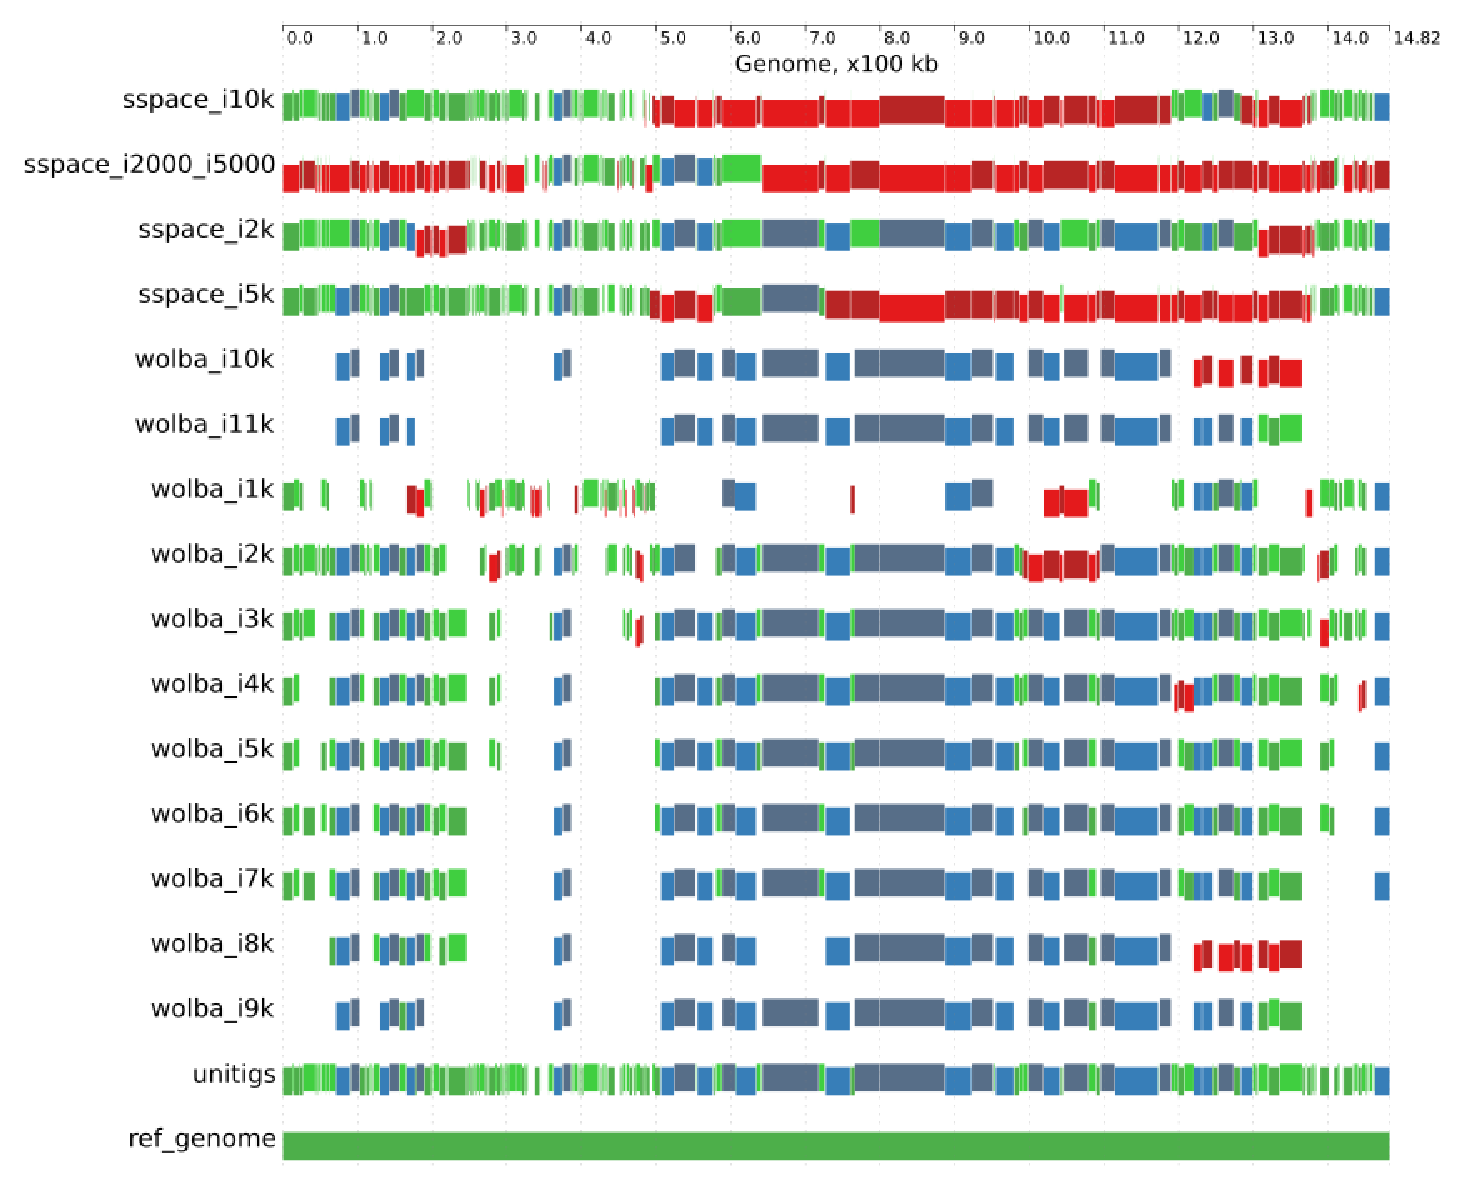
\includegraphics[scale=0.7]{alignment_woinserts}
}
\end{center}
\caption{Alignment of scaffolding solutions on the reference genome of Wolbachia endosymbiont}
\scriptsize This plot shows alignment of contigs to the reference genome and positions of misassemblies in these scaffolds. Correctly aligned big ($>$ 10kb) scaffolds are blue if the boundaries agree, and green if the boundaries don't agree. Scaffolds containing an important amount of misassemblies are red. Here, SSPACE solution with the 2kbp insert size library shows the less misassembled regions with the most reference coverage. However the solution is broken up in an enormous amount of scaffolds (336), most of them being just the unsucessfully attached small unitigs. SSPACE also fails to produce any valid scaffold for the genomic regions containing the large $>$5000 repeats (see their exact coordinates in table \ref{tab:repeatcoord}).
\label{fig:alignwoinsert}
\end{figure}


\begin{table}[h!]
\centering
\resizebox{10cm}{!}{
\begin{tabular}{|l|l|l|l|l|l|l|}
\hline
{[}S1{]} & {[}E1{]} & {[}S2{]} & {[}E2{]} & {[}LEN 1{]} & {[}LEN 2{]} & {[}\% IDY{]}  \\ \hline
1        & 1482355  & 1        & 1482355  & 1482355     & 1482355     & 100.00        \\
118235   & 119770   & 14639    & 13104    & 1536        & 1536        & 99.67          \\
951662   & 953006   & 62728    & 61384    & 1345        & 1345        & 100.00         \\
13104    & 14639    & 119770   & 118235   & 1536        & 1536        & 99.67          \\
295130   & 296467   & 156339   & 155002   & 1338        & 1338        & 100.00         \\
1044418  & 1046269  & 178963   & 177112   & 1852        & 1852        & 100.00         \\
295131   & 296471   & 201307   & 199967   & 1341        & 1341        & 99.93          \\
\rowcolor{red!10}
346054   & 354494   & 259128   & 250682   & 8441        & 8447        & 99.56          \\
1040287  & 1042282  & 286820   & 284825   & 1996        & 1996        & 100.00        \\
1370666  & 1372235  & 293326   & 291757   & 1570        & 1570        & 99.87          \\
886392   & 887730   & 296467   & 295129   & 1339        & 1339        & 100.00         \\
\rowcolor{red!10}
1459215  & 1461421  & 296650   & 294476   & 2207        & 2175        & 98.50          \\
\rowcolor{red!10}
353564   & 355681   & 325239   & 323122   & 2118        & 2118        & 97.54          \\
\rowcolor{red!10}
346054   & 351130   & 332648   & 327572   & 5077        & 5077        & 99.94          \\
\rowcolor{red!10}
250682   & 259128   & 354494   & 346054   & 8447        & 8441        & 99.56          \\
295130   & 296467   & 426552   & 425215   & 1338        & 1338        & 100.00         \\
353564   & 355681   & 449855   & 447738   & 2118        & 2118        & 97.54          \\
951661   & 953011   & 506502   & 505152   & 1351        & 1351        & 99.93          \\
1305338  & 1306686  & 553913   & 552565   & 1349        & 1349        & 99.93          \\
295129   & 296467   & 887730   & 886392   & 1339        & 1339        & 100.00         \\
505152   & 506502   & 953011   & 951661   & 1351        & 1351        & 99.93          \\
284825   & 286820   & 1042282  & 1040287  & 1996        & 1996        & 100.00         \\
177112   & 178963   & 1046269  & 1044418  & 1852        & 1852        & 100.00         \\
1334495  & 1335840  & 1306687  & 1305342  & 1346        & 1346        & 100.00         \\
1305342  & 1306686  & 1320819  & 1319475  & 1345        & 1345        & 100.00         \\
1305342  & 1306687  & 1335840  & 1334495  & 1346        & 1346        & 100.00         \\
291757   & 293326   & 1372235  & 1370666  & 1570        & 1570        & 99.87          \\
\rowcolor{red!10}
294476   & 296650   & 1461421  & 1459215  & 2175        & 2207        & 98.50         \\ \hline
\end{tabular}
%\footnotesize{Notes}
\caption{Coordinates and length of repeats in the \textit{Wolbachia endosymbiont} genome}
\label{tab:repeatcoord}
}
\end{table}


\clearpage
%-------------------------------------------------------------------------------
% BODEH!
%-------------------------------------------------------------------------------
\section{Discussion}
\section{Conclusion}
\clearpage

%-------------------------------------------------------------------------------
%BIBLIOGRAPHY
%-------------------------------------------------------------------------------
\pagenumbering{gobble}
\section{References}
\bibliography{scaffoldingbiblio, scaffoldingbiblio_non_articles}
\bibliographystyle{naturemag}
%\printbibliography
\newpage
\section{Annexes}
\label{sec:anx}
\setcounter{figure}{0}
\renewcommand{\thefigure}{\Alph{figure}}
 

\end{document}